\documentclass[a4paper]{ctexart}

\usepackage{listings} 
\usepackage{geometry}
\usepackage{booktabs}
\usepackage{graphicx}
\usepackage{tabularx}
\usepackage{multirow}
\usepackage{enumitem}
\usepackage{subcaption}
\usepackage{adjustbox}
\usepackage{array}
\usepackage{float}
\usepackage{longtable}
\usepackage[dvipsnames]{xcolor}

\newcolumntype{P}[1]{>{\centering\arraybackslash}m{#1}}

\renewcommand{\multirowsetup}{\centering}

\geometry{
    a4paper,
    left=23mm,
    right=23mm,
    top=23mm,
    bottom=23mm,
}

\title{HE保险平台系统 需求规格说明书}
\author{
  曾少勋 171250603\\
  刘洪禹 171840773\\
  黄国钊 171250530\\
  夏雨笛 171250011\\
}
\date{\today}

\begin{document}

\maketitle

\begin{abstract}
  本项目为 CodeOcean 小组在 2020 春季学期《需求与商业模式设计》课程大作业中所设计的同名项目,此文档为其需求规格说明书,记录了系统的功能描述及需求。本小组通过分工完成了分析模型的建立与分析、需求追踪、需求规格说明的撰写工作,本篇文档主要分为三部分:1-3节为需求规格说明书,第4节为用于分析需求的模型,第5节为工作中为追踪需求所建立的跟踪矩阵。
\end{abstract}

\tableofcontents

\newpage

\section{引言}

\subsection{目的}

本⽂档描述了HE保险平台系统的功能需求和⾮功能需求,HE保险平台是一个网上的保险信息整合与交流平台。后续展开开发实现与验证工作时,开发团队会以此⽂档为依据。

\subsection{范围}

本文档要描述的是HE保险平台系统的需求说明,预期中的中的功能包括浏览各种保险信息与排名、获得保险推荐、保险的购买、理赔与咨询、以及与其他用户交流保险信息。该产品可以为用户提供一个信息查询的平台,同时也可以提供简化后保险服务的流程办理,目的是节省用户整合保险信息的成本,提供相互交流渠道,同时也为保险公司拓宽销售通路。

\subsection{定义、首字母缩写和缩略词}
\subsubsection{定义}
\begin{itemize}
    \item \textbf{普通用户}:以购买保险或查询保险信息为目标的系统用户。
    \item \textbf{客服}:包括平台自身的工作人员与领域专家,回复普通用户关于平台使用或保险服务的问题。
\end{itemize}

\subsection{参考文献}

\begin{enumerate}
  \item IEEE 标准
  \item "HE保险平台" 需求获取文档
  \item 《需求工程——软件建模与分析》
\end{enumerate}

\section{总体描述}

\subsection{项目前景}

\subsubsection{背景与机遇}

在现实生活中,保险是一个对每个人来说十分重要的商品,但是除了农保社保医保等这些统一收费的保险产品,还可能遇到车险,财险等保险,而这些需要私人考察和购买的保险产品。对于这些产品,消费者者只能通过保险宣传册或者推销员来了解相应的保险,了解渠道十分有限。如果消费者要比较不同公司的相应产品来找到最适合自己的一款,需要符出很多的精力。其次,购买了一家的产品后,如果同时又需要其他类型的保险产品,为了避免麻烦,往往会在同一家公司购买,就有可能错过更好的产品。如果某一天用户需要购买保险,他需要询问相应的推销员,再到线下柜台办理手续,有时甚至需要推销员上门讲解和收取材料,大大增加了保险购买周期的时长。

该产品所要打入的是国内的保险市场,由于我国的保险密度较低,而且我国的经济还在高速发展中,所以国内保险市场还尚未饱和。用户通过“HE保险平台系统”查看各公司的保险信息,并可以进一步进行购买和理赔。该系统为客户提供了整合后的保险信息,简化后的购买和理赔流程,以及用户可以相互交流的平台,能大大降低用户选择、购买和理赔的成本。目前虽然也有一些在线保险平台,但大多数都是保险公司自己推出的平台,在信息密度和客观性上都不能满足我们的目标群体的需求,因此该系统有较为开朗的前景。在市场趋势上,人口老龄化可以为保险带来机遇;当前国内保险意识依然偏弱,但人均保费收入增长十分快速,说明市场还有待挖掘。技术上,首先各种商业模式的互联网化趋势十分明显,很多保险公司都推出了线上平台提供服务,并且应用机器学习和自动化流程降低成本;鉴于保险平台需要特殊的安全性,区块链技术已经开始被应用到保险公司的工作流程中,避免虚假索赔和欺诈造成的巨大损失。企业战略上,保险公司也倾向于提供自助的服务提高用户理赔体验,另外也开始寻求销售渠道多样化,通过多种合作关系增加自家保险的覆盖面与销售额。为了保证该系统能提供完整的服务,系统需要依赖成熟的软件开发与维护技术、数据分析技术、适合线上平台的简化的保险购买和理赔流程建模、运营该系统的运维、客服等人力资源、运行系统的服务器资源、提供保险来源的保险公司合作关系等技术或者资源。

\subsubsection{业务需求}

\begin{itemize}
  \item \textbf{BO-1}:在第一版应用之后的3个月内,将用户的平均保险挑选时间降低50\%。
  \item \textbf{BO-2}:在在第一版应用之后的3个月内,将用户的平均保险业务办理时间降低30\%。
  \item \textbf{BO-3}:在第一版应用之后的6个月内,将合作保险公司的保险销售额提升15\%。
  \item \textbf{SC-1}:在第一版应用之后的6个月内,用户对在本系统中所办理的保险业务的好评率达到85\%。
  \item \textbf{SC-2}:在第一版应用之后的6个月内,与本平台进行合作的保险公司数量达到当前市场中的80\%(以市场份额作为基准)。
\end{itemize}

\subsection{商品功能}

该系统主要围绕着想买保险或者不明确自己是否应该买保险的用户提供服务,包括浏览信息 、购买与理赔、咨询三大块,其中浏览信息的方式可以有直接查看、查看推荐或者在论坛讨论等多种方式,最后将其细分为以下功能:

\begin{itemize}
  \item \textbf{FE-1}:浏览各公司所提供的险种和详细信息。
  \item \textbf{FE-2}:浏览险种综合排名。
  \item \textbf{FE-3}:根据自身情况,获得推荐险种。
  \item \textbf{FE-4}:对险种进行购买。
  \item \textbf{FE-5}:在线申请理赔。
  \item \textbf{FE-6}:在线与保险公司客服交流或咨询。
  \item \textbf{FE-7}:通过平台,与其他用户交流保险经验和信息。
\end{itemize}

\subsection{用户特征}

\subsubsection{用户识别} 总的来说,该系统的用众有:普通用户、平台工作人)、保险公司、领域专家(顾问和咨询)。

进一步,用户可以分为三类:一类是普通用户,他们可能已经明确了对保险的购买需求,或者仍对保险是否适合自己抱有疑问;另一类是保险公司,他们需要查看平台上自家产品的购买与评价情况;还有最后一类主要指平台的客服人员和后台管理员,他们是系统的管理者,他们负责平台日常的运维、解答一些用户在平台使用上的疑问。

\subsubsection{用户描述} 针对上一小节用户识别的结果,对每一类用户描述如下:

\begin{itemize}
  \item \textbf{普通用户}:这类用户可能有明确的购保意愿,或者对于保险的作用心存疑惑,不理解保险对于自己的收益,或者详细流程,难以判断自己是否需要购入保险。他们使用平台的目的是希望利用获得保险相关的知识,或是专业人士的建议。
  \item \textbf{保险公司}:与平台合作的保险公司(的数据分析人员),他们需要掌握自家产品的销售情况,或者了解别的公司的动向以及时调整销售策略,因此使用该平台是希望得到自家产品的数据汇总,以及查看别的公司的评价情况。
  \item \textbf{平台工作人员和管理员}:工作人员和管理员是平台的管理者,他们负责解答普通用户对于平台使用的问题,或是反馈bug。他们中的部分是人工客服,和用户直接接触。他们或许有工作经历,但是对于平台的使用还需要培训以达到熟练完成事务的处理。
  \item \textbf{领域专家}:这类专家有着丰富的保险行业的知识,在系统中担任回应普通用户关于保险的咨询。

\end{itemize}

\begin{adjustbox}{width=\columnwidth,center}
  \centering
  \begin{tabular}{|m{2cm}|m{3cm}|m{2cm}|m{4cm}|m{3cm}|}
    \hline
    涉众 & 主要目标 & 教育水平 & 主要关注点 & 使用能力 \\
    \hline
    普通用户 & 选择一款最合适自己的保险,明确自己是否需要购买保险 & 不等。 & 希望交互流程简捷方便,元素设计清晰易懂。 & 可能不能熟练使用互联网产品。 \\
    \hline
    保险公司 & 查看自家产品数据,了解别家产品评价 & 较高。 & 平台易于使用,数据汇报清晰直观。 & 一般。 \\
    \hline
    平台工作人员和管理员 & 平台运维,解答用户使用过程中的问题 & 不等。 & 平台要易于使用,能方便查看用户信息。 & 需要培训到较为熟练水平。 \\
    \hline
    领域专家 & 顾问,提供专业知识的支持 & 较高。 & 平台能提供完整的沟通渠道,保证能顺利沟通。 & 一般。 \\
    \hline
  \end{tabular}
\end{adjustbox}

\subsection{约束}

\begin{enumerate}[label=CON\arabic*.]
  \item 系统前端应基于 Web 技术,后端使用 Java 开发。
  \item 开发过程应使用螺旋模型。
  \item 代码提交前必须通过风格检查。
\end{enumerate}

\subsection{假设与依赖}

\begin{itemize}
  \item \textbf{AS-1}:承载系统的服务器有较高的稳定性,操作系统为CentOS。
  \item \textbf{AS-2}:服务器所在的网络是安全的。
  \item \textbf{DE-1}:系统的推荐功能依赖于用户提供与保险公司提供的信息与数据。
\end{itemize}

\section{详细需求描述}

\subsection{对外接口需求}

\subsubsection{用户界面}

\begin{figure}[H]
  \centering
  \begin{minipage}[t]{0.3\textwidth}
  \centering
  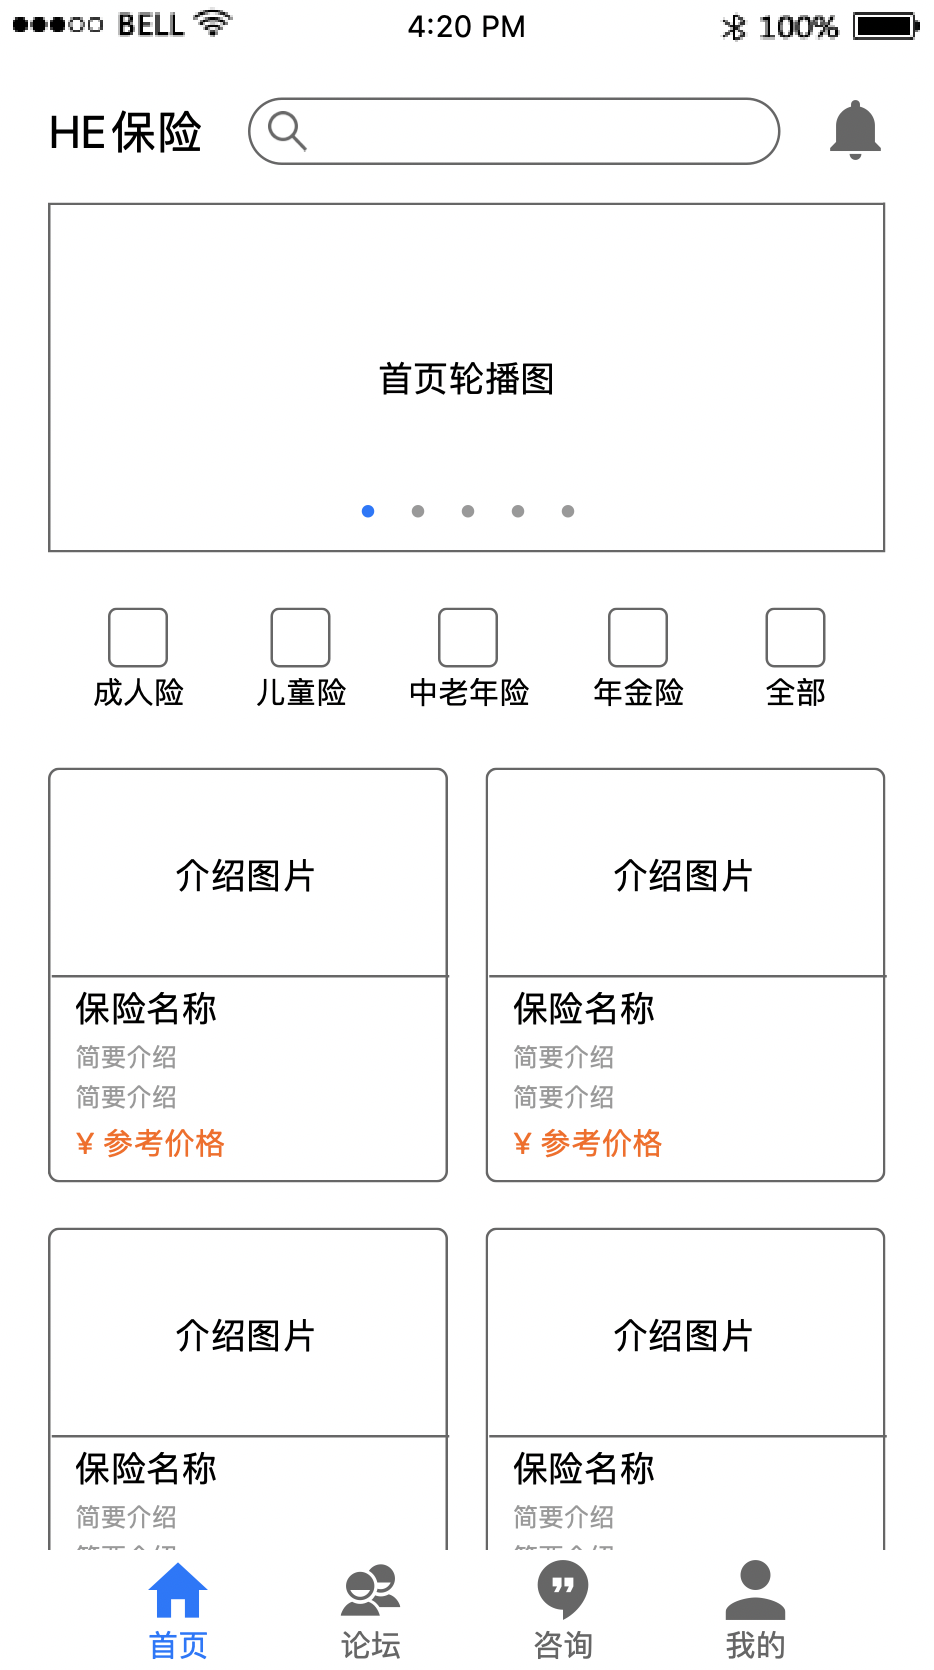
\includegraphics[width=0.9\textwidth]{prototype1}
  \caption{首页}
  \end{minipage}
  \begin{minipage}[t]{0.3\textwidth}
  \centering
  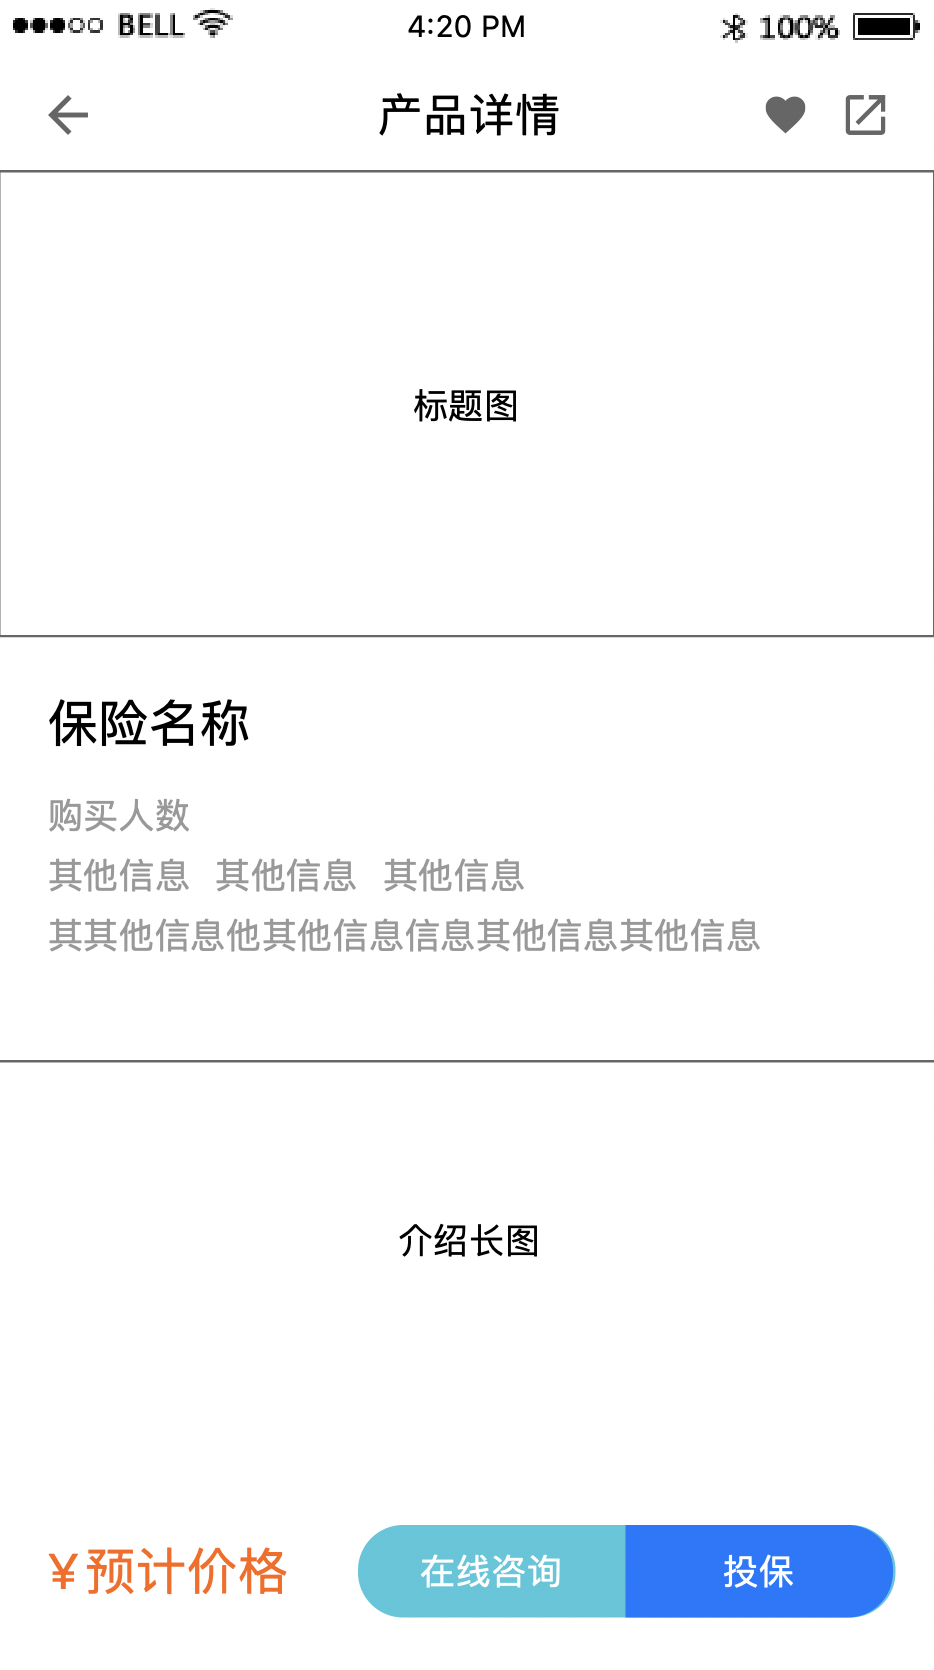
\includegraphics[width=0.9\textwidth]{prototype2}
  \caption{产品详情}
  \end{minipage}
  \begin{minipage}[t]{0.3\textwidth}
  \centering
  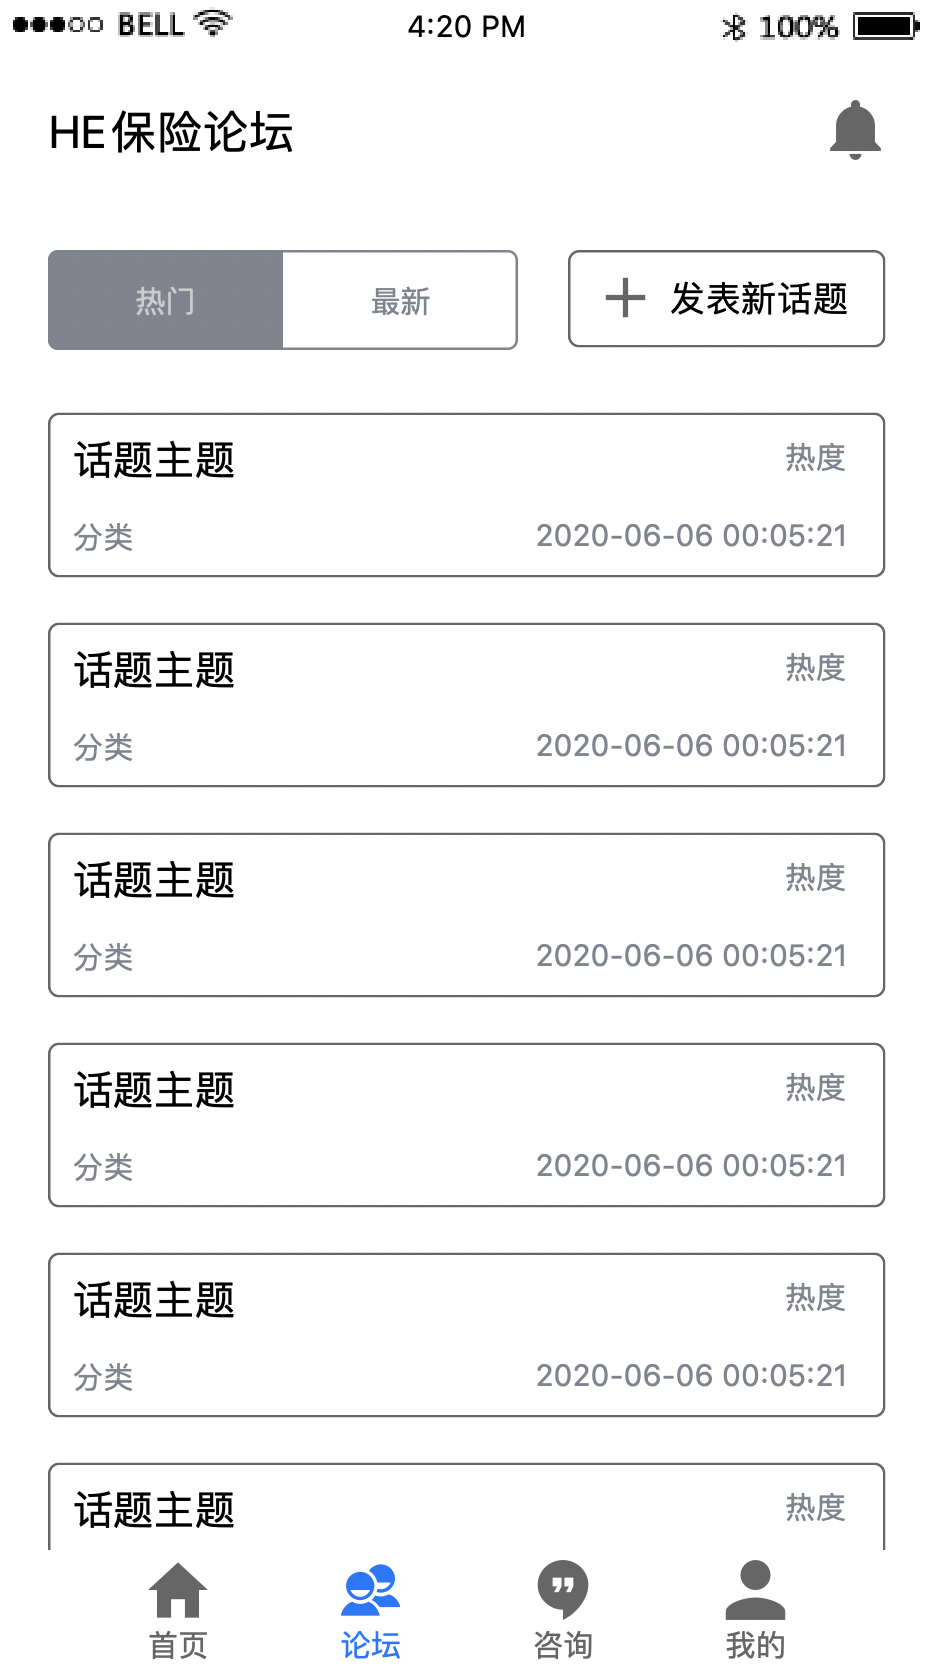
\includegraphics[width=0.9\textwidth]{prototype3}
  \caption{保险论坛}
  \end{minipage}
\end{figure}
\begin{figure}[H]
  \centering
  \begin{minipage}[t]{0.3\textwidth}
  \centering
  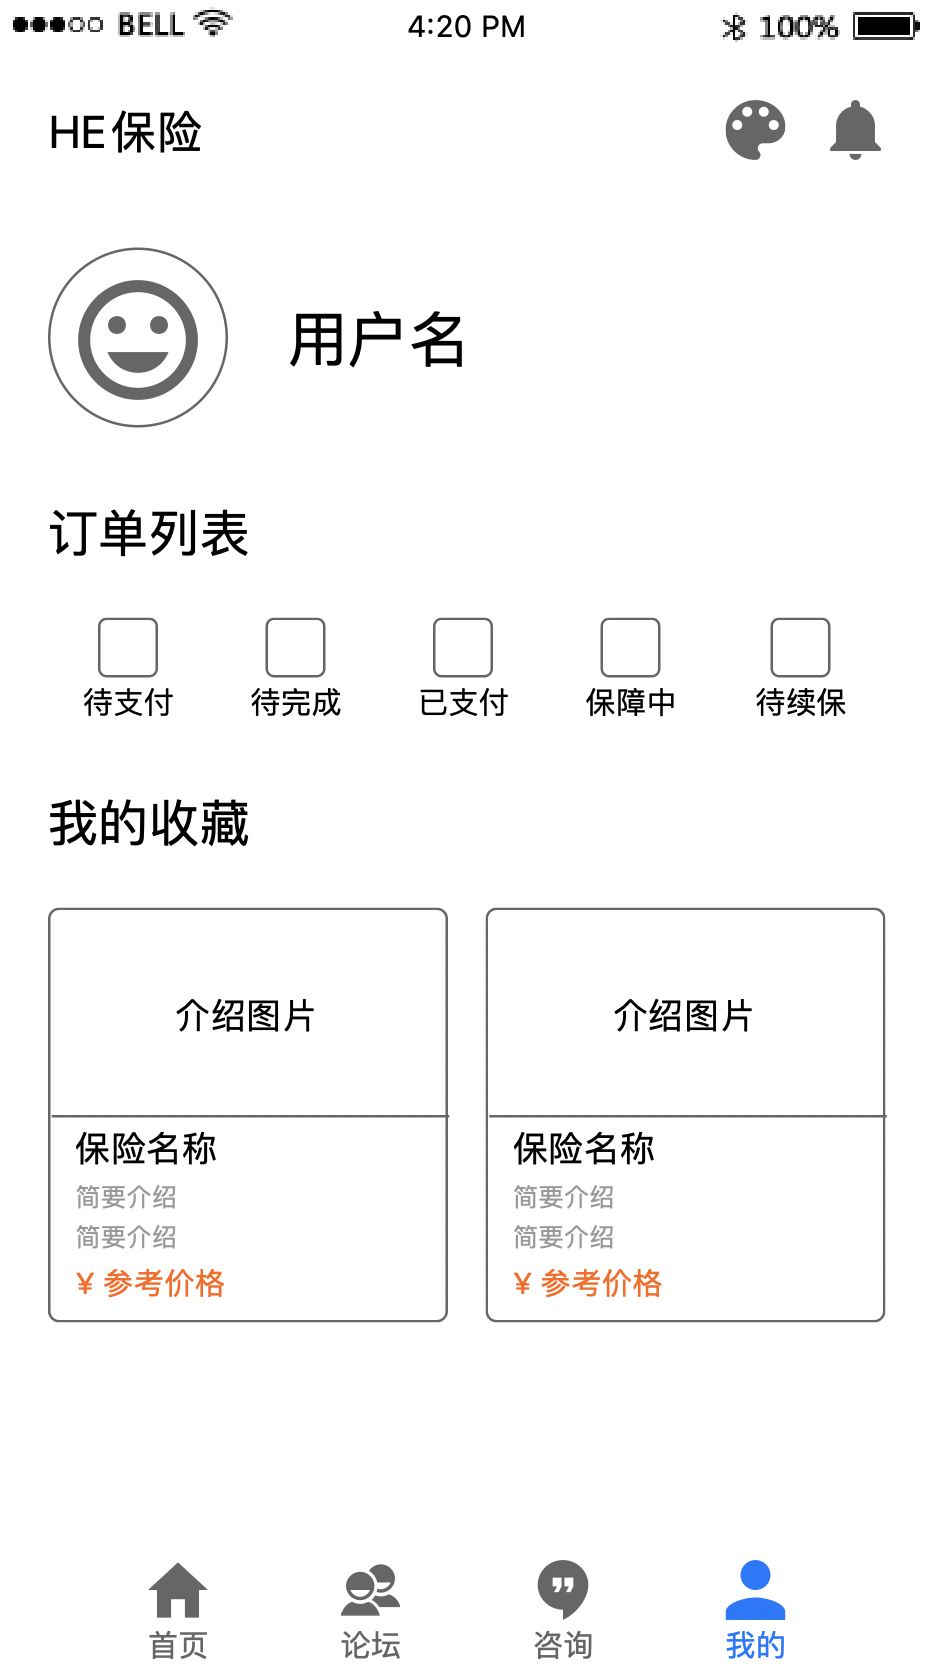
\includegraphics[width=0.9\textwidth]{prototype4}
  \caption{用户信息}
  \end{minipage}
  \begin{minipage}[t]{0.3\textwidth}
  \centering
  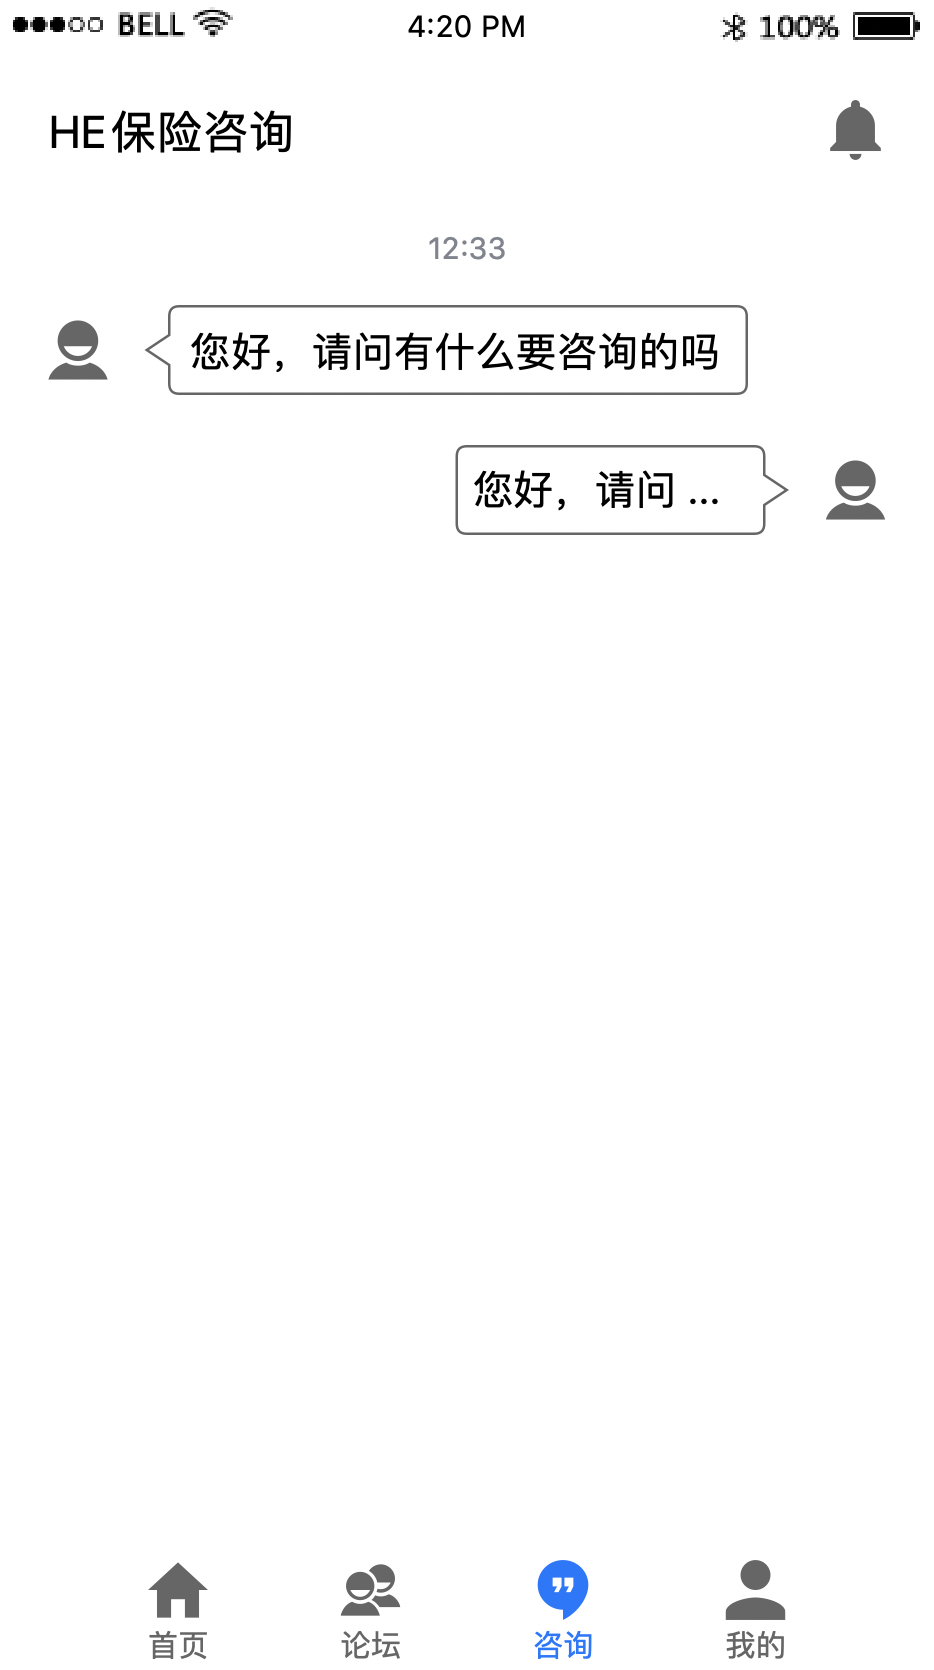
\includegraphics[width=0.9\textwidth]{prototype5}
  \caption{客服界面}
  \end{minipage}
\end{figure}

\subsubsection{软件接口}

平台和第三方支付平台之间通过网络双向通信,第三方支付平台用于支付,将用户支付成功与否的信息返回给平台。

平台和保险公司之间通过网络双向通信,用于转交用户材料,以及保险公司回复受理结果。

\subsubsection{硬件接口}

系统采用分布式开发,部署在多台服务器上,数据库多实例应保障数据一致性。

\subsubsection{通信接口}

用户浏览器、移动端app与后端使用基于 json 的 REST API 进行通信 

系统和保险公司之间使用基于 json 的 REST API 进行通信


\subsection{功能需求}

\subsubsection{申请理赔}

\paragraph{特征描述}

申请理赔是本系统的主要功能,用户在购买保险之后,可能会有理赔需求。此时用户需要登录系统,提交材料,由系统审核之后交由保险公司进行处理,并将处理之后的结果返回给用户。

\paragraph{刺激 / 响应序列}

\begin{itemize}
  \item 刺激: 用户申请理赔
  \item 响应: 系统显示理赔步骤,并提供提交材料入口
  \item 刺激: 用户提交材料
  \item 响应: 系统上传材料并通知管理员
  \item 刺激: 管理员审核材料后允许申诉
  \item 响应: 系统将材料发送给相应的保险公司
  \item 刺激: 管理员审核材料后驳回申诉
  \item 响应: 系统通知用户申诉失败
\end{itemize}

\paragraph{相关功能需求}

\begin{center}
  \begin{tabular}{p{6cm}|p{8cm}}
    \toprule
    Apply.Upload         & 用户上传材料      \\
    \midrule
    Apply.Audit & 管理员审核 \\
    \midrule
    Apply.Send            & 系统发送文件给第三方保险公司                      \\
    \midrule
    Apply.Receive            & 系统接受第三方保险公司发送的结果文件                      \\
    \midrule
    Apply.Persist            & 系统记录此次理赔过程                      \\
    \midrule
    Apply.Notify            & 系统告知用户理赔结果                    \\
    \bottomrule
  \end{tabular}
\end{center}

\subsubsection{购买保险}

\paragraph{特征描述}

购买保险是系统的核心功能之一,目的是允许用户方便、快捷、安全的购买保险产品。

\paragraph{刺激 / 响应序列}

\begin{itemize}
  \item 刺激: 用户进入购买页面
  \item 响应: 系统能够展示各个种类的保险
  \item 刺激: 用户点击某项保险进行购买
  \item 响应: 系统请求第三方接口负责支付,结束后将结果展示给用户
  \item 刺激: 第三方接口返回用户支付完成信息
  \item 响应: 系统接受信息并根据返回情况来判断用户是否成功支付购买
\end{itemize}

\paragraph{相关功能需求}

\begin{center}
  \begin{tabular}{p{6cm}|p{8cm}}
    \toprule
    Buy.Show & 用户进入购买页面,系统展示各个种类的保险,数据定义详见数据需求 \\
    \midrule
    Buy.Pay  & 用户点击购买,系统请求第三方支付接口,并跳转到对应的支付页面,用户完成支付后,将根据第三方接口的返回情况来判断是否支付成功,以此判断此次购买成功与否                                      \\
    \midrule
    Buy.Persist   &  系统记录此次购买过程和结果            \\
    \bottomrule
  \end{tabular}
\end{center}

\subsubsection{联系客服}

\paragraph{特征描述}

用户在使用系统的过程中,如果产生疑问,可以申请人工答疑。

\paragraph{刺激 / 响应序列}

\begin{itemize}
  \item 刺激: 用户发起提问
  \item 响应: 系统展示历史问题列表
  \item 刺激: 用户选择查看某个历史问题详情
  \item 响应: 系统展示历史问题详情
  \item 刺激: 用户要求提出新的问题
  \item 响应: 系统展示供用户输入问题的入口
  \item 刺激: 用户描述问题并提交
  \item 响应: 系统显示提交成功,并通知客服人员
  \item 刺激: 客服人员和用户沟通
  \item 响应: 系统提供沟通入口
\end{itemize}

\paragraph{相关功能需求}

\begin{center}
  \begin{tabular}{p{6cm}|p{8cm}}
    \toprule
    Oncall.History & 系统展示历史问题列表 \\
    \midrule
    Oncall.Upload & 用户新建新问题 \\
    \midrule
    Oncall.Communicate & 用户和人工客服进行双向沟通 \\
    \midrule
    Oncall.Persist & 系统记录此次用户咨询过程 \\
    \bottomrule
  \end{tabular}
\end{center}

\subsubsection{浏览保险信息}

\paragraph{特征描述}

浏览保险信息是本系统的基础功能。用户可以查看系统整合后的保险信息,并可以进行诸如筛选和对比等额外操作,以满足了解保险信息的需求。

\paragraph{刺激 / 响应序列}

\begin{itemize}
  \item 刺激: 用户请求保险信息
  \item 响应: 系统分页显示完全保险信息列表
  \item 刺激: 用户请求推荐保险信息
  \item 响应: 系统分页显示为该用户推荐的保险信息列表
  \item 刺激: 用户输入搜索关键字,或者选择筛选保险所属公司
  \item 响应: 系统根据条件过滤不符合条件的保险信息,显示新列表
  \item 刺激: 用户选择某个保险信息条目
  \item 响应: 系统展示该保险的详细信息,包括保险名、所属公司、价格、详细条款、用户评价。
  \item 刺激: 用户选择另一条保险信息条目请求对比。
  \item 响应: 系统同时展示两种保险的详细信息,对齐条目提供信息对比。
\end{itemize}

\paragraph{相关功能需求}

\begin{center}
    \begin{tabular}{p{6cm}|p{8cm}}
      \toprule
      Insurance.Info.Request & 系统应该允许用户请求完全保险列表或者推荐保险列表 \\
      Insurance.Info.Full & 系统读取完全保险信息列表      \\
      Insurance.Info.Recommend & 系统选择推荐保险信息列表 \\
      \midrule
      Insurance.Codition.Input & 系统应该允许用户输入搜索关键字或者选择保险所属公司\\
      Insurance.Codition.Filter & 系统根据筛选条件对保险信息列表进行筛选 \\
      \midrule
      Insurance.Choose & 系统应该允许用户选择保险条目 \\
      Insurance.Detail & 系统展示保险条目详细信息 \\
      \midrule
      Insurance.Detail.Choose & 系统应该允许用户在展示保险信息详情的时候选择另外的保险进行信息对比 \\
      Insurance.Detail.Compare  & 系统对比保险详细信息                      \\
      \bottomrule
    \end{tabular}
\end{center}

\subsubsection{浏览论坛}

\paragraph{特征描述}
用户可以在论坛上浏览帖子,参与对保险的讨论,或者查看别的用户对某款保险的评价。


\paragraph{刺激 / 响应序列}

\begin{itemize}
  \item 刺激: 用户请求帖子列表
  \item 响应: 系统分页显示完全帖子列表,用户可以看见主题与一楼正文
  \item 刺激: 用户请求推荐帖子列表
  \item 响应: 系统分页显示为该用户推荐的帖子列表,用户可以看见主题与一楼正文
  \item 刺激: 用户输入搜索关键字
  \item 响应: 系统根据条件过滤不含关键字的帖子,显示新列表
  \item 刺激: 用户选择某个帖子
  \item 响应: 系统显示帖子详细内容,包括主题、正文、以及回帖
\end{itemize}

\paragraph{相关功能需求}

\begin{center}
    \begin{tabular}{p{6cm}|p{8cm}}
      \toprule
      Post.Info.Request & 系统应该允许用户请求完全帖子列表或者推荐帖子列表 \\
      Post.Info.Full & 系统读取完全帖子列表      \\
      Post.Info.Recommend & 系统选择推荐帖子列表 \\
      \midrule
      Post.Keyword.Input & 系统应该允许用户输入搜索关键字\\
      Post.Keyword.Filter & 系统根据关键字对帖子列表进行筛选 \\
      \midrule
      Post.Choose & 系统应该允许用户选择帖子条目 \\
      Post.Detail & 系统展示帖子内容 \\
      \bottomrule
    \end{tabular}
\end{center}

\subsubsection{发帖}

\paragraph{特征描述}
用户可以在论坛上发布帖子,询问保险相关问题或者分享保险体验经验。

\paragraph{刺激 / 响应序列}

\begin{itemize}
  \item 刺激: 用户请求发帖
  \item 响应: 系统显示编辑界面,供用户输入内容
  \item 刺激: 用户输入帖子主题与正文
  \item 响应: 系统实时更新编辑结果
  \item 刺激:用户选择将某款保险或者自己发布过的某次保险评价关联
  \item 响应:系统显示关联的保险或者评价。
  \item 刺激: 用户选择发布帖子
  \item 响应: 系统提交帖子并显示提交结果
\end{itemize}

\paragraph{相关功能需求}

\begin{center}
    \begin{tabular}{p{6cm}|p{8cm}}
      \toprule
      Post.Edit.Request & 系统应该允许用户请求发布帖子 \\
      Post.Edit.Show & 系统显示帖子编辑界面     \\
      \midrule
      Post.Content.Input & 系统应该允许用户输入帖子内容\\
      \midrule
      Post.Link.Input & 系统应该允许用户选择关联的保险或者评价 \\
      \midrule
      Post.Submit & 系统应该允许用户发布帖子 \\
      Post.Submit.Result & 系统显示发布结果 \\
      \bottomrule
    \end{tabular}
\end{center}

\subsubsection{回帖}

\paragraph{特征描述}
用户可以在论坛上对帖子进行回复,以进行相互交流。

\paragraph{刺激 / 响应序列}

\begin{itemize}
  \item 刺激: 用户请求回帖
  \item 响应: 系统显示编辑界面,供用户输入内容
  \item 刺激: 用户输入回帖那日容
  \item 响应: 系统实时更新编辑结果
  \item 刺激: 用户选择发布回帖
  \item 响应: 系统提交回帖并显示提交结果
\end{itemize}

\paragraph{相关功能需求}

\begin{center}
    \begin{tabular}{p{6cm}|p{8cm}}
      \toprule
      Reply.Request & 系统应该允许用户请求回帖 \\
      Reply.Edit.Show & 系统显示回帖编辑界面     \\
      \midrule
      Reply.Content.Input & 系统应该允许用户输入回帖内容\\
      \midrule
      Reply.Submit & 系统应该允许用户发布回帖 \\
      Reply.Submit.Result & 系统显示发布结果 \\
      \bottomrule
    \end{tabular}
\end{center}


\subsubsection{用户评价}

\paragraph{特征描述}

用户在进行完购买、理赔或者咨询的服务之后,需要对服务进行评价。

\paragraph{刺激 / 响应序列}

\begin{itemize}
    \item 刺激:用户发起评价
    \item 响应:系统展示评价编辑页面
    \item 刺激:用户打分,编写评价
    \item 响应:系统实时保存评价内容至草稿箱
    \item 刺激:用户提交评价
    \item 响应:系统将用户评价存入数据库中
\end{itemize}

\paragraph{相关功能需求}

\begin{center}
  \begin{tabular}{p{6cm}|p{8cm}}
    \toprule
    Comment.List        & 获取用户的评价列表 \\
    \midrule
    Comment.Save      & 暂时保存用户的评价至草稿箱           \\
    \midrule
    Comment.Submit & 用户提交评价,系统将评价持久化到数据库           \\
    \midrule
    Comment.Delete & 用户删除自己的评价           \\
    \midrule
    Comment.Edit & 用户修改自己的评价          \\
    \bottomrule
  \end{tabular}
\end{center}

\subsubsection{用户咨询}

\paragraph{特征描述}

用户在使用平台或者在购买保险的过程中,如果遇到困难,可以联系客服或者保险专家进行解答。

\paragraph{刺激 / 响应序列}

\begin{itemize}
    \item 刺激:用户发起咨询
    \item 响应:系统展示咨询的界面
    \item 刺激:用户选择咨询客服
    \item 响应:系统为用户自动匹配空闲客服
    \item 刺激:用户选择咨询领域专家
    \item 响应:系统展示专家列表
    \item 刺激:用户选择咨询领域专家
    \item 响应:系统展示专家列表
    \item 刺激:用户预约领域专家空闲时间
    \item 响应:系统提示领域专家
\end{itemize}

\paragraph{相关功能需求}

\begin{center}
  \begin{tabular}{p{6cm}|p{8cm}}
    \toprule
    Consult.Select        & 选择咨询服务 \\
    \midrule
    Consult.FreeTime      & 系统为用户匹配空闲时间的客服           \\
    \midrule
    Consult.List & 系统展示领域专家列表           \\
    \midrule
    Consult.Detail & 系统展示领域专家的详细信息           \\
    \midrule
    Consult.Book & 用户预约领域专家          \\
    \midrule
    Consult.Inform & 提示领域专家工作时间          \\
    \bottomrule
  \end{tabular}
\end{center}

\subsubsection{用户管理}

\paragraph{特征描述}

管理员可以利用平台管理用户。

\paragraph{刺激 / 响应序列}

\begin{itemize}
    \item 刺激:管理员添加用户
    \item 响应:系统在用户列表中添加用户
    \item 刺激:管理员修改用户信息
    \item 响应:系统在用户列表中修改用户信息
    \item 刺激:管理员删除用户
    \item 响应:系统在用户列表中删除用户
    \item 刺激:管理员提交修改
    \item 响应:系统将用户列表的更新同步到数据库
    \item 刺激:管理员查询筛选用户
    \item 响应:系统返回符合要求的用户
\end{itemize}

\paragraph{相关功能需求}

\begin{center}
  \begin{tabular}{p{6cm}|p{8cm}}
    \toprule
    UserManager.Add        & 用户列表中添加用户 \\
    \midrule
    UserManager.Edit      & 用户列表中修改用户信息           \\
    \midrule
    UserManager.Delete & 用户列表中删除用户           \\
    \midrule
    UserManager.Submit & 管理员提交用户列表的修改,同步到数据库           \\
    \midrule
    UserManager.Search & 管理员搜索筛选用户          \\
    \bottomrule
  \end{tabular}
\end{center}


\subsubsection{产品信息管理}

\paragraph{特征描述}

管理员、保险公司在平台上新建、编辑产品,产品信息包括:标题大图、介绍长图、保险名称、保险类型、保险价格、保险合同样本等。

\paragraph{刺激 / 响应序列}

\begin{itemize}
    \item 刺激:管理员、保险公司选择新建产品
    \item 响应:系统提供新产品表单
    \item 刺激:管理员、保险公司选择修改产品
    \item 响应:系统提供产品表单,其中包含当前产品信息
    \item 刺激:管理员、保险公司填写产品表单
    \item 响应:系统进行校验,并显示校验结果,确保用户输入的合法性
    \item 刺激:管理员、保险公司提交表单
    \item 响应:系统记录操作日志、持久化储存产品信息、并提示用户操作结果
\end{itemize}

\paragraph{相关功能需求}

\begin{center}
  \begin{tabular}{p{6cm}|p{8cm}}
    \toprule
    ProductManager.Add        & 管理员、保险公司新建产品 \\
    \midrule
    ProductManager.Edit       & 管理员、保险公司编辑产品 \\
    \midrule
    ProductManager.Verify & 系统校验用户填写的表单           \\
    \midrule
    ProductManager.Submit & 管理员、保险公司提交表单           \\
    \midrule
    ProductManager.Log & 系统记录操作日志          \\
    \bottomrule
  \end{tabular}
\end{center}

\subsubsection{查看产品购买记录}

\paragraph{特征描述}

管理员、保险公司、客服可以在平台上查询产品购买记录,包括:保险名称、购买时间、购买人基本信息、所签合同、评价等信息。

\paragraph{刺激 / 响应序列}

\begin{itemize}
    \item 刺激:管理员、保险公司、客服选择查询条件
    \item 响应:系统显示符合条件的购买记录
    \item 刺激:管理员、保险公司、客服选择排序方式
    \item 响应:系统显示排序后的购买记录
\end{itemize}

\paragraph{相关功能需求}

\begin{center}
  \begin{tabular}{p{6cm}|p{8cm}}
    \toprule
    OrderManager.Search        & 管理员、保险公司、客服搜索产品购买记录 \\
    \midrule
    OrderManager.Sorter       & 管理员、保险公司、客服选择产品排序条件 \\
    \bottomrule
  \end{tabular}
\end{center}

\subsubsection{查看产品评价}

\paragraph{特征描述}

普通用户可以在平台上看到其他用户关于产品的评价。

\paragraph{刺激 / 响应序列}

\begin{itemize}
    \item 刺激:普通用户选择对应商品,查看评价
    \item 响应:系统显示该商品的用户评价
    \item 刺激:普通用户选择评价关键字(如理赔、家庭等)
    \item 响应:系统显示包含此关键字的评价
    \item 刺激:普通用户选择评价类型(好评、中评、差评)
    \item 响应:系统显示此类型的评价
    \item 刺激:普通用户选择评价排序方式(时间优先、有用优先)
    \item 响应:系统显示排序后的评价
\end{itemize}

\paragraph{相关功能需求}

\begin{center}
  \begin{tabular}{p{6cm}|p{8cm}}
    \toprule
    VoteManager.List        & 普通用户查看产品评价 \\
    \midrule
    VoteManager.Filter        & 普通用户对产品评价过滤 \\
    \midrule
    VoteManager.Sorter        & 普通用户对产品评价排序 \\
    \bottomrule
  \end{tabular}
\end{center}



\subsection{非功能需求}

\subsubsection{易用性}

\begin{enumerate}[label=Usability\arabic*.]
  \item 智能推荐和推送给用户相关消息。
  \item 专业的保险术语有标注和解释供用户阅读和理解。
  \item 初次使用系统的用户应能自行根据提示进行操作。
  \item 系统应支持不同尺寸的屏幕。
\end{enumerate}

\subsubsection{可修改性}

\begin{enumerate}[label=Modifiability\arabic*.]
  \item 当保险策略发生更改时,系统管理员应能在 5 小时内完成数据更新。
  \item 当有新的保险数据来源时,系统管理员应能在 1 日内完成数据接入。
\end{enumerate}

\subsubsection{可靠性}

\begin{enumerate}[label=Reliability\arabic*.]
  \item 系统每年不可用时间不得超过 3h。
\end{enumerate}

\subsubsection{性能}

\begin{enumerate}[label=Performance\arabic*.]
  \item 系统首页的打开时间不应超过 2s。
  \item 系统每秒钟至少能处理 1000 个搜索请求。
\end{enumerate}

\subsubsection{约束}

\begin{enumerate}[label=IC\arabic*.]
  \item 保护用户个人信息,防止信息泄漏,维护用户隐私权。
\end{enumerate}

\subsection{数据需求}

\subsubsection{数据定义}

\begin{enumerate}[label=DR\arabic*.]
  \item 保险信息
        \begin{center}
          \begin{tabular}{llll}
            \toprule
            字段           & 类型              & 描述                       & 默认值   \\
            \midrule
            id             & \texttt{string}   & 保险 id,在全系统中唯一    &          \\
            name           & \texttt{string}   & 保险名称                   & 空字符串 \\
            company        & \texttt{string}   & 所属保险公司               & 空列表   \\
            startTime      & \texttt{integer}  & 该项保险策略开始时间       & 0        \\
            endTime        & \texttt{integer}  & 该项保险策略结束时间       & 0        \\
            detail         & \texttt{string}   & 保险详细信息,包括理赔策略 & 空字符串 \\
            \bottomrule
          \end{tabular}
        \end{center}
        
  \item 购买信息
    \begin{center}
      \begin{tabular}{llll}
        \toprule
        字段           & 类型              & 描述                       & 默认值   \\
        \midrule
        id             & \texttt{string}   & 订单 id,在全系统中唯一    &          \\
        name           & \texttt{string}   & 订单名称                   & 空字符串 \\
        time           & \texttt{integer}  & 订单生成时间               & 0        \\
        price          & \texttt{string}   & 订单价格                   & 空字符串 \\
        uid            & \texttt{string}   & 购买用户id                 & 空字符串 \\
        gid            & \texttt{string}   & 保险id                     & 空字符串 \\
        \bottomrule
      \end{tabular}
        \end{center}
        
  \item 用户信息
    \begin{center}
      \begin{tabular}{llll}
        \toprule
        字段           & 类型              & 描述                       & 默认值   \\
        \midrule
        id             & \texttt{string}   & 用户 id,在全系统中唯一    &          \\
        name           & \texttt{string}   & 用户名称                   & 空字符串 \\
        time           & \texttt{integer}  & 注册时间。                 & 0        \\
        gender         & \texttt{string}   & 性别                       & 空字符串 \\
        year           & \texttt{string}.  & 年龄                       & 空字符串 \\
        phone          & \texttt{string}   & 电话                       & 空字符串 \\
        \bottomrule
      \end{tabular}
    \end{center}
    
\end{enumerate}

\subsection{其他}

\subsubsection{安装需求}

\begin{enumerate}[label=Install\arabic*.]
  \item 在安装系统时,需初始化导入一些初始化保险数据。
\end{enumerate}

\section{分析模型}
\subsection{申请理赔}
图\ref{fig:申请理赔类图}描述了申请理赔过程中的类关系。
\begin{figure}[H]
\centering
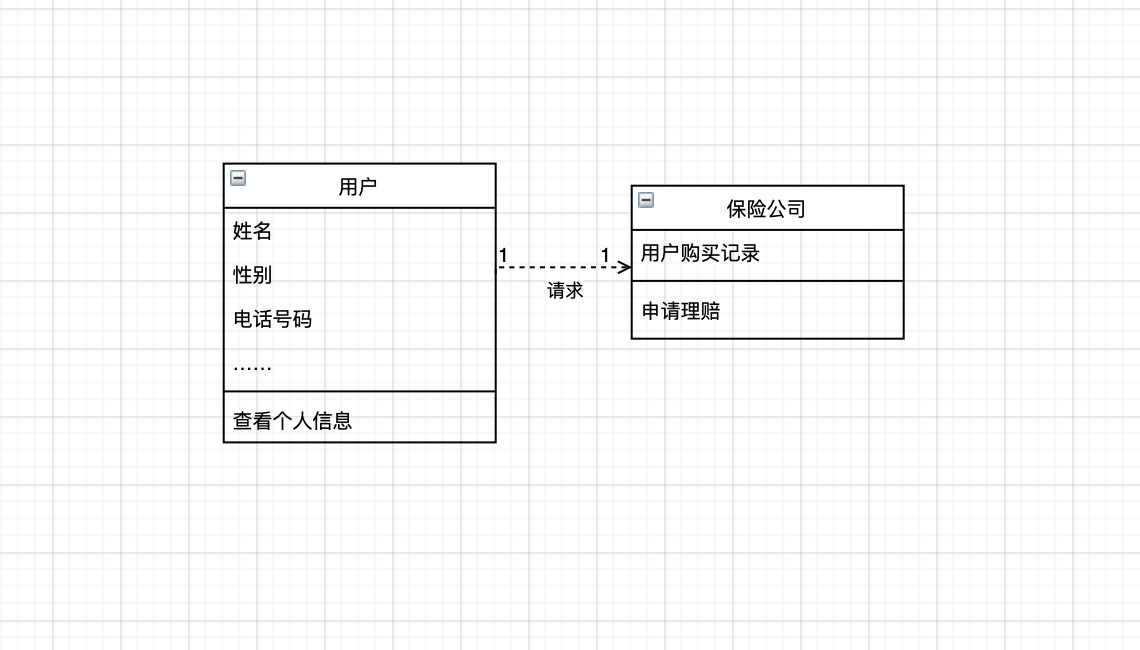
\includegraphics[scale=0.3]{image/1_6类图.png}
\caption{申请理赔类图}
\label{fig:申请理赔类图}
\end{figure}
该图由用户、保险公司2个类共同组成。用户和保险公司之间的关系是请求和被请求。用户类存储个人的基本信息,同时提供接口以供查看个人信息;保险公司保存各个用户的购买记录,同时提供接口供用户申请理赔。注意:平台会在中间起到中转的作用,用户并不是直接请求保险公司,而是递交材料给平台,平台负责请求保险公司。考虑到平台本身在这个过程中只是中间转手,因此不特地画出一个类。 \\

图\ref{fig:申请理赔顺序图}描述了申请理赔过程中用户和系统的交互过程序列
\begin{figure}[H]
\centering
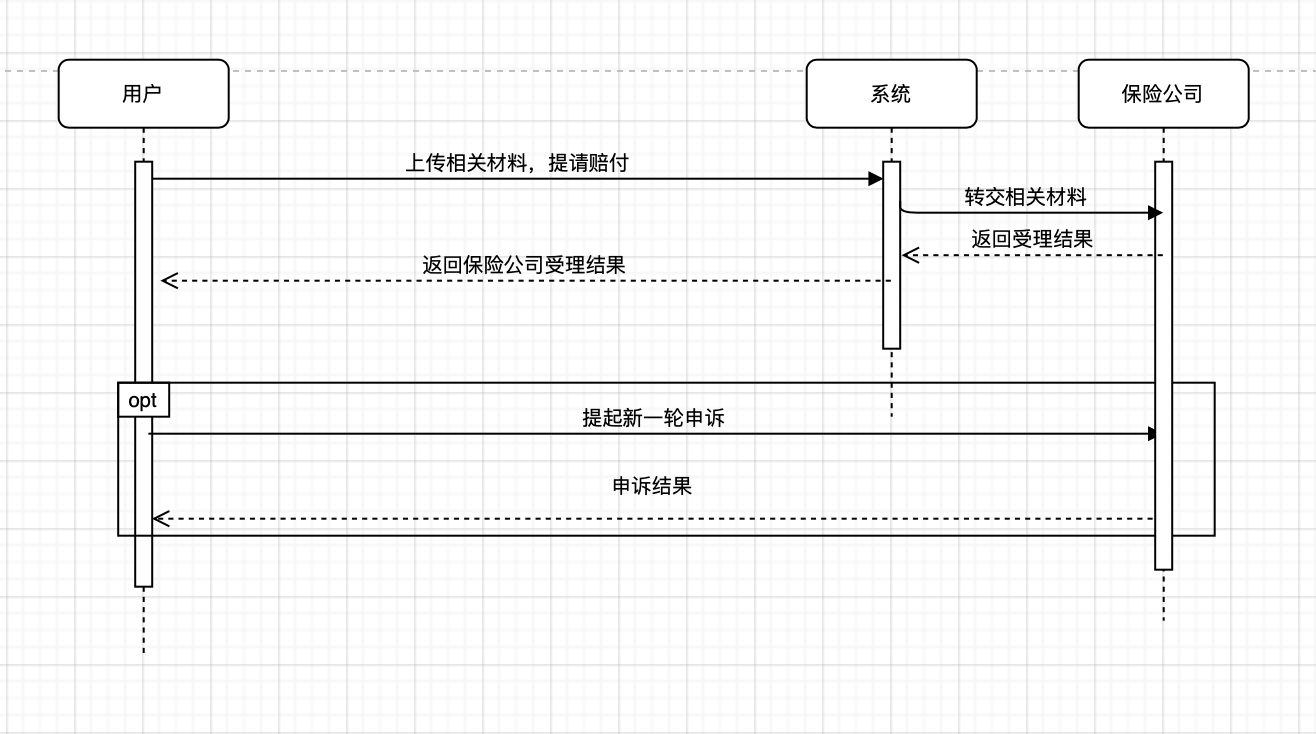
\includegraphics[scale=0.5]{image/1_2顺序图.png}
\caption{申请理赔顺序图}
\label{fig:申请理赔顺序图}
\end{figure}
该顺序图记录了用户申请理赔的过程。大致分为两个部分,首先是平台中间负责转交材料,其后如果用户对于理赔结果不满意可以和公司进行交涉和申诉。\\

图\ref{fig:申请理赔状态图}描述了申请理赔过程中状态和流转情况。
\begin{figure}[H]
\centering
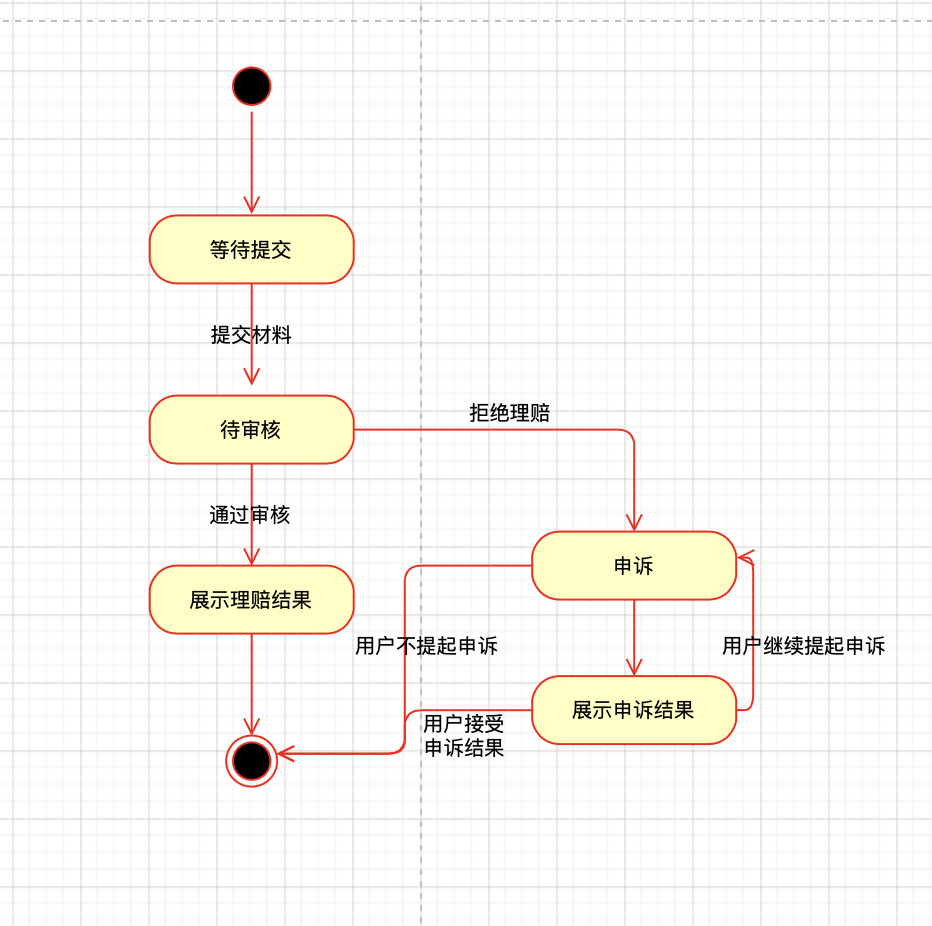
\includegraphics[scale=0.3]{image/1_8状态图.png}
\caption{申请理赔状态图}
\label{fig:申请理赔状态图}
\end{figure}
该状态图记录了用户理赔过程中的一系列状态变化,包括提交等待状态等。注意有个分叉流程就是如果用户拒绝接收保险公司的理赔结果,那么可以反复提出申诉,这个过程平台并不直接参与。
\subsection{购买保险}
图\ref{fig:购买保险类图}描述了购买保险过程的类关系。
\begin{figure}[H]
\centering
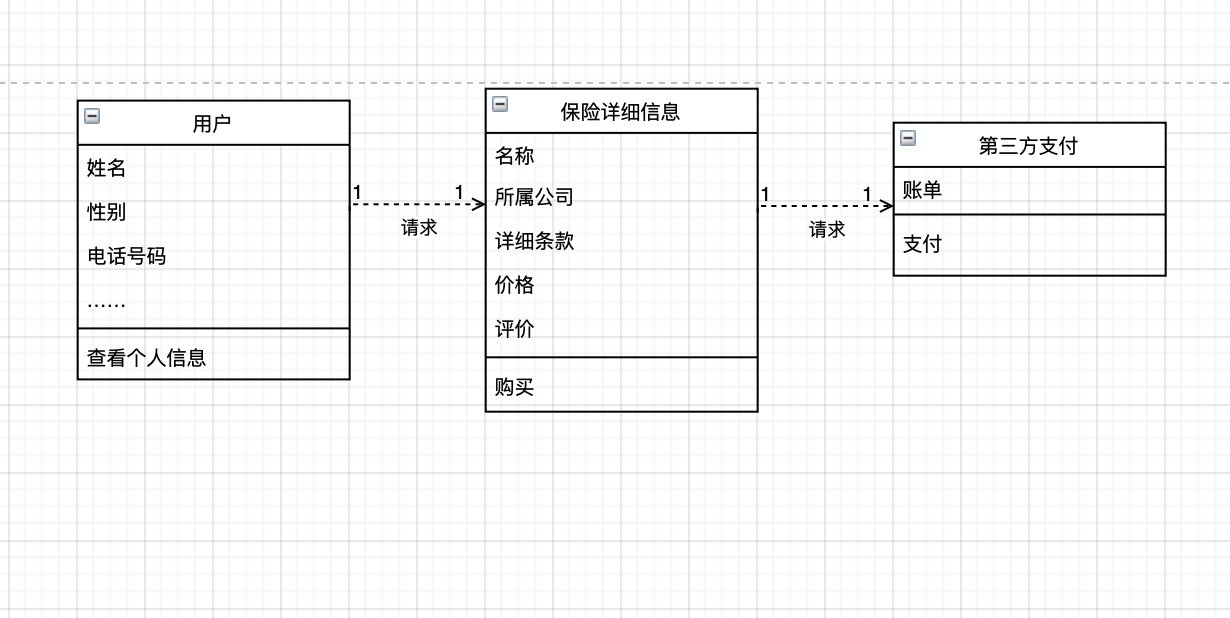
\includegraphics[scale=0.5]{image/1_5类图.png}
\caption{购买保险类图}
\label{fig:购买保险类图}
\end{figure}
该图由用户、保险公司、第三方支付平台3个类共同组成。用户包括个人信息,以及提供查看个人信息的接口;平台主要负责展示保险信息以及提供购买功能,具体的支付功能转交给第三方支付平台来完成。\\

图\ref{fig:购买保险顺序图}描述了购买保险过程中用户和系统的交互过程序列。
\begin{figure}[H]
\centering
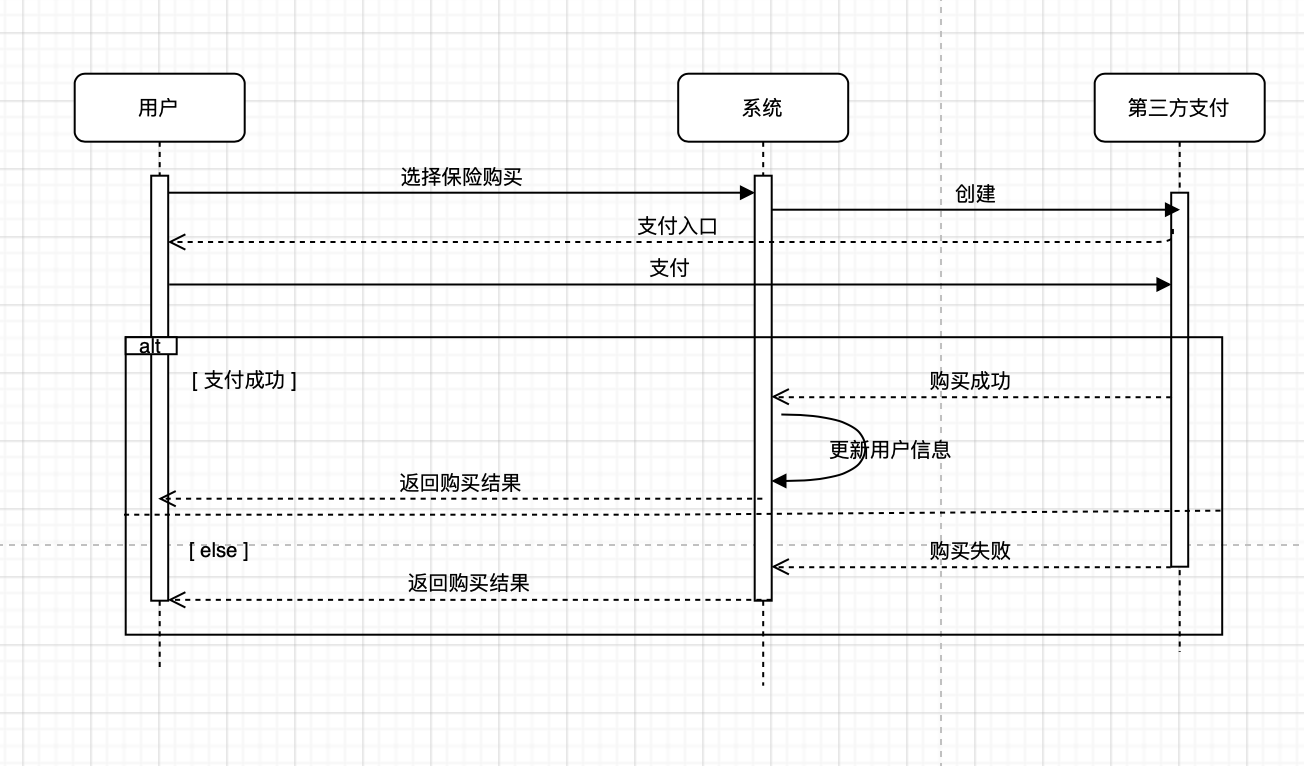
\includegraphics[scale=0.5]{image/1_3顺序图.png}
\caption{购买保险顺序图}
\label{fig:购买保险顺序图}
\end{figure}
该顺序图展示了用户购买保险的过程。用户在系统上选择保险进行购买,具体的支付功能交由第三方支付平台来完成。注意:平台要根据第三方支付接口返回的结果来判断支付成功或失败,以此来决定此次购买的结果,并做持久化记录。\\

图\ref{fig:购买保险状态图}描述了购买保险过程中状态和流转情况。
\begin{figure}[H]
\centering
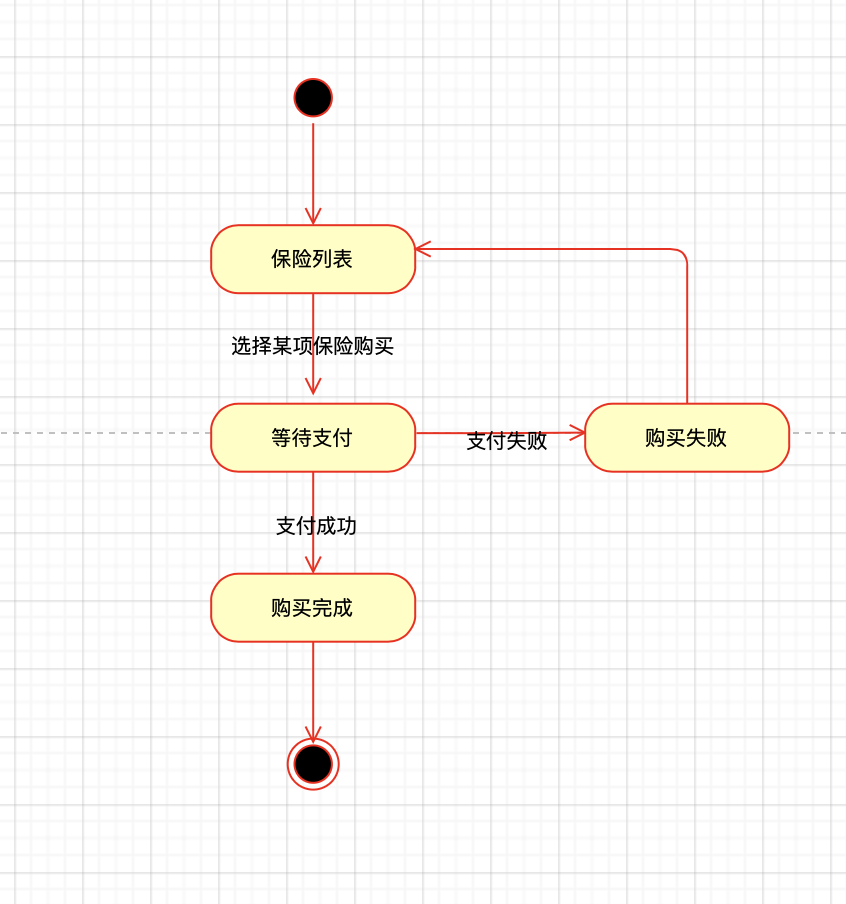
\includegraphics[scale=0.3]{image/1_9状态图.png}
\caption{购买保险状态图}
\label{fig:购买保险状态图}
\end{figure}
该状态图显示了用户购买保险过程中出现的状态和流转情况。注意支付成功与否的信息是从第三方接口获得的。
\subsection{联系客服}
图\ref{fig:联系客服类图}描述了联系客服过程的类关系
\begin{figure}[H]
\centering
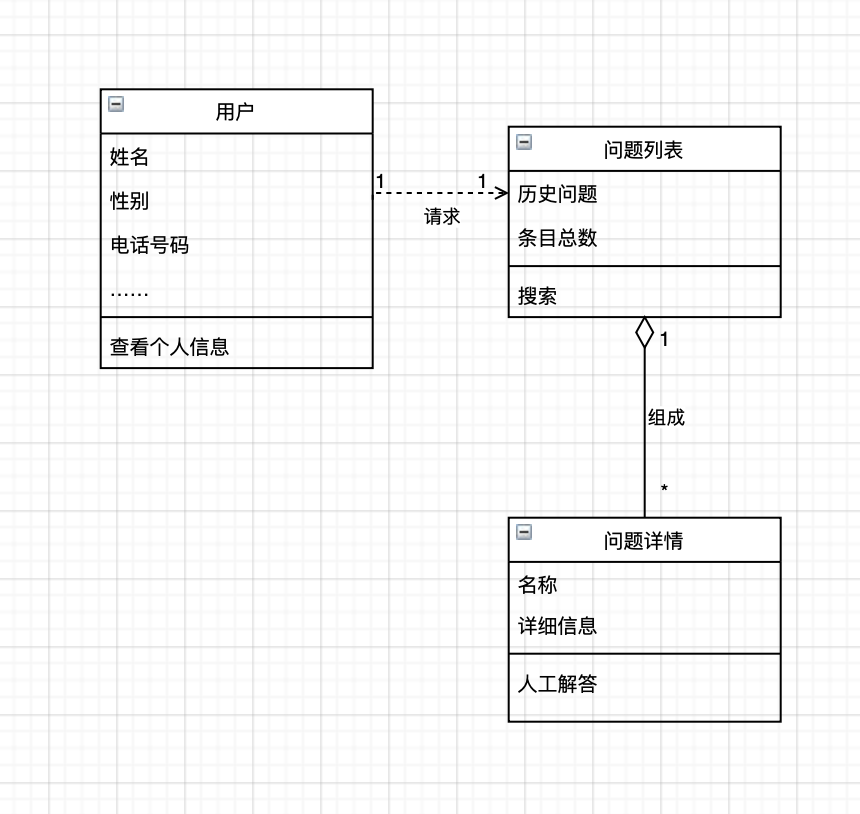
\includegraphics[scale=0.3]{image/1_7类图.png}
\caption{联系客服类图}
\label{fig:联系客服类图}
\end{figure}
该图由用户、问题列表、问题详情3个类共同组成。主要关注问题列表和问题详情,问题详情组成了问题列表。在问题详情中,有人工解答这个行为,目的是在用户搜索历史问题还没得到解答的时候,可以提请人工客服来解答。\\

图\ref{fig:联系客服顺序图}描述了联系客服过程中用户和系统的交互过程序列。
\begin{figure}[H]
\centering
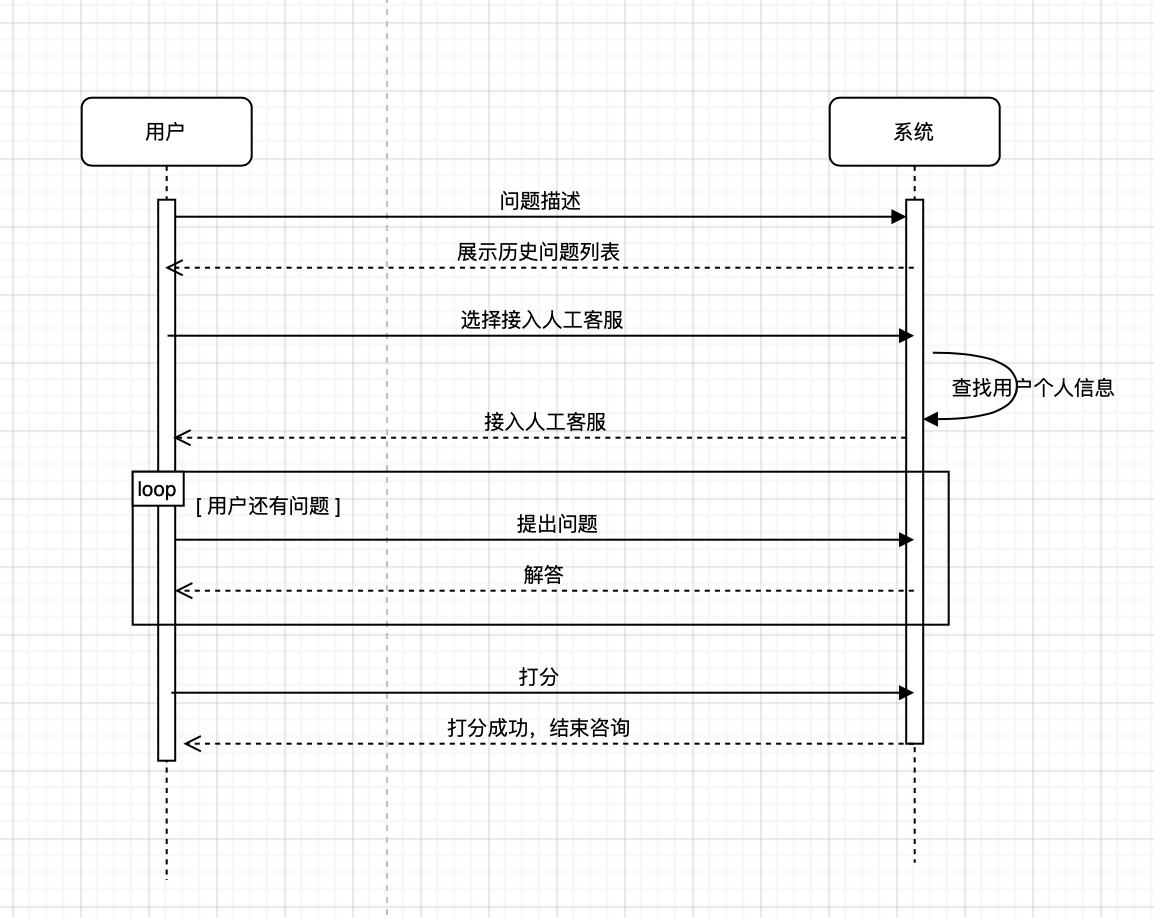
\includegraphics[scale=0.4]{image/1_4顺序图.png}
\caption{联系客服顺序图}
\label{fig:联系客服顺序图}
\end{figure}
该图展示了用户联系客服的整个流程。用户在搜索问题之后,如果还没能得到满意的解答,可以提请人工客服解答。与人工客服的交流是对话问答式,直到解决了用户的问题为止。\\

图\ref{fig:联系客服状态图}描述了联系客服过程中状态和流转情况。
\begin{figure}[H]
\centering
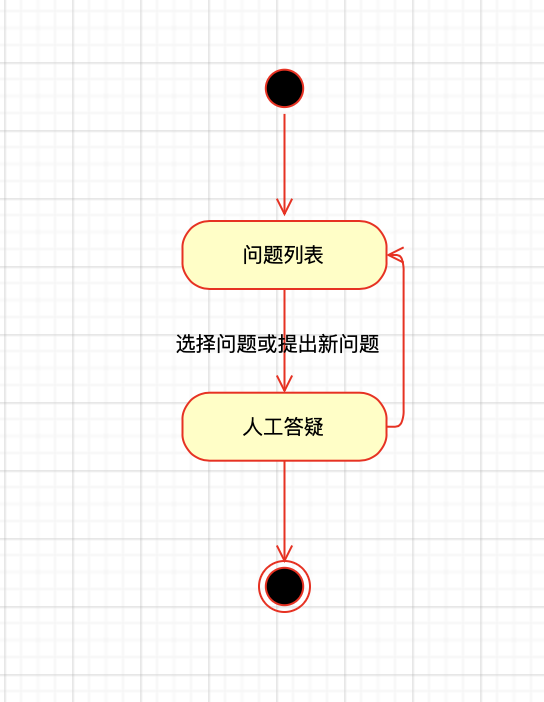
\includegraphics[scale=0.4]{image/1_10状态图.png}
\caption{联系客服状态图}
\label{fig:联系客服状态图}
\end{figure}
该图展示了用户联系客服中的状态和流转情况。是一个循环的过程,在历史问题和人工客服解答之间循环,知道解决用户的问题。
\subsection{浏览保险信息}
图\ref{fig:浏览保险信息类图} 描述浏览保险信息的需求相关的实体的属性和交互。
\begin{figure}[H]
\centering
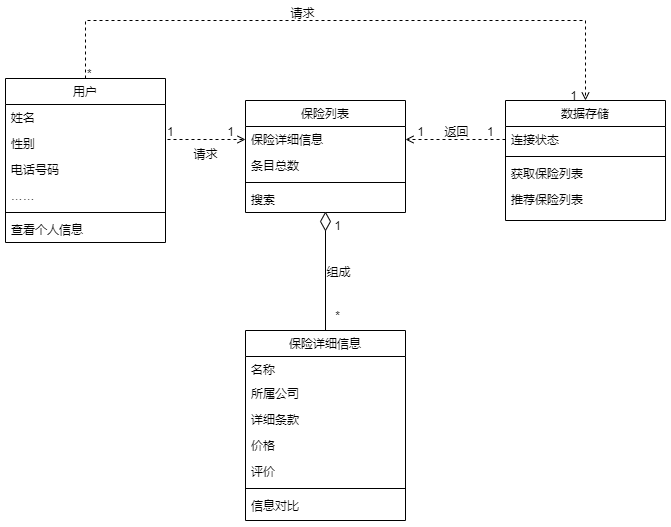
\includegraphics[scale=0.4]{image/2_2类图.png}
\caption{浏览保险信息类图}
\label{fig:浏览保险信息类图}
\end{figure}
该图由用户、保险列表、保险详细信息、数据存储4类共同组成。数据存储作为数据提供者,可以获取一般保险列表或者推荐保险列表。保险列表除了将一些保险信息作为属性,还会有一些额外属性,并且有搜索筛选功能。保险详细信息之间可以进行对比。\\

图\ref{fig:浏览保险信息顺序图}描述了浏览保险信息需求中的实体交互顺序。
\begin{figure}[H]
\centering
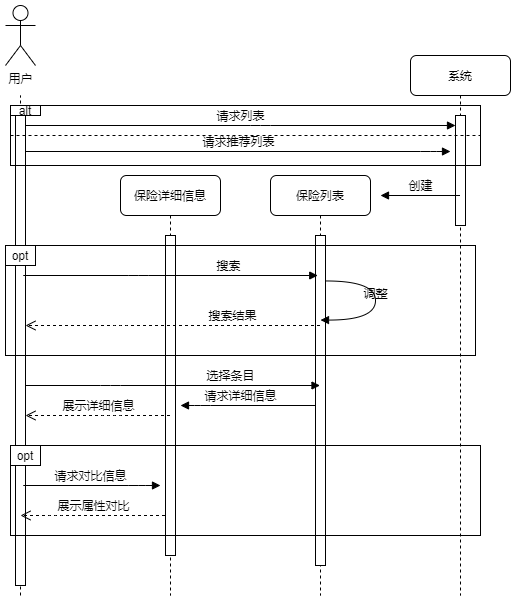
\includegraphics[scale=0.4]{image/2_3顺序图.png}
\caption{浏览保险信息顺序图}
\label{fig:浏览保险信息顺序图}
\end{figure}
在图中,用户先向系统获取保险列表(通过请求一般列表或者推荐列表),可选地对列表进行关键词搜索或者条件筛选保险列表。查看保险详细信息之后,可以可选地对感兴趣的保险信息的属性进行对比。\\

图\ref{fig:浏览保险信息状态图}描述了浏览保险信息需求中所经过的状态和转移。
\begin{figure}[H]
\centering
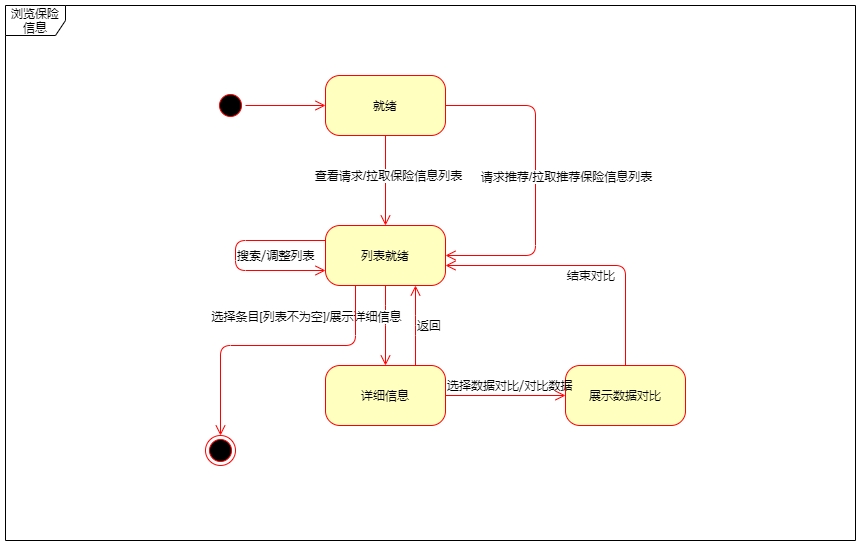
\includegraphics[scale=0.4]{image/2_4状态图.png}
\caption{浏览保险信息状态图}
\label{fig:浏览保险信息状态图}
\end{figure}
状态主要有就绪、列表就绪、展示详细信息、展示数据对比四种。在预想中列表就绪是一个主干状态,要浏览详细信息或者进行数据对比都需要经过列表就绪状态。数据对比状态需要经过详细信息状态,与顺序图的交互顺序一致.

\subsection{浏览帖子/发帖/回帖}
图\ref{fig:浏览帖子信息类图}描述浏览帖子信息的需求相关的实体的属性和交互。
\begin{figure}[H]
\centering
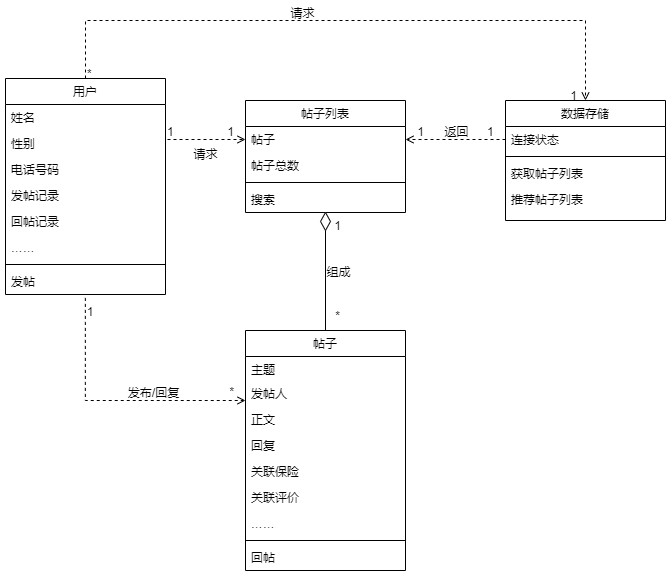
\includegraphics[scale=0.4]{image/2_5类图.png}
\caption{浏览帖子信息类图}
\label{fig:浏览帖子信息类图}
\end{figure}
该图与浏览保险信息类图类似,由用户、帖子列表、帖子和数据存储4类共同组成。除了与浏览保险信息类图相似的部分,用户还可以进行发帖或者回帖。\\

图\ref{fig:浏览帖子信息顺序图}描述浏览帖子信息需求中的实体交互顺序。
\begin{figure}[H]
\centering
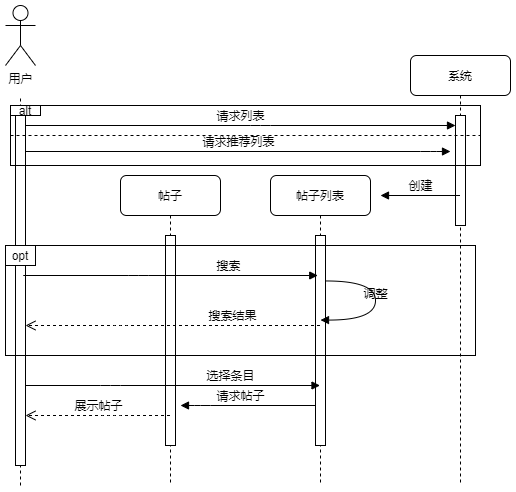
\includegraphics[scale=0.4]{image/2_6顺序图.png}
\caption{浏览帖子信息顺序图}
\label{fig:浏览帖子信息顺序图}
\end{figure}
在图中,用户先向系统获取帖子列表(通过请求一般列表或者推荐列表),可选地对列表进行关键词搜索来筛选保险列表。\\

图\ref{fig:发帖顺序图}描述发帖需求中的实体交互顺序。
\begin{figure}[H]
\centering
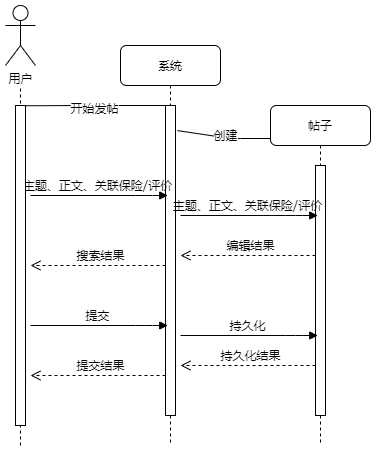
\includegraphics[scale=0.5]{image/2_7顺序图.png}
\caption{发帖顺序图}
\label{fig:发帖顺序图}
\end{figure}
在该图中,用户与系统交互,通过系统设置帖子的各个属性,最终提交,由系统进行持久化,用户获得持久化的结果。\\

图\ref{fig:回帖顺序图}描述回帖需求中的实体交互顺序。
\begin{figure}[H]
\centering
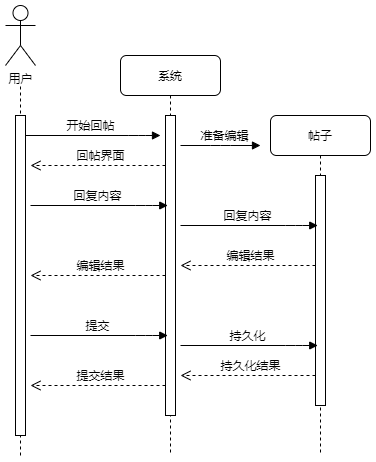
\includegraphics[scale=0.5]{image/2_8顺序图.png}
\caption{回帖顺序图}
\label{fig:回帖顺序图}
\end{figure}
与发帖顺序图不同的是,系统此时读取已持久化的帖子,准备编辑信息。用户完成编辑后提交,由系统进行持久化,返回结果。因为回帖是与浏览帖子的联系并不紧密,因此两个需求的顺序图分开来画。\\

图\ref{fig:浏览帖子与回帖状态图}描述浏览帖子信息与回帖需求中所经过的状态和转移。
\begin{figure}[H]
\centering
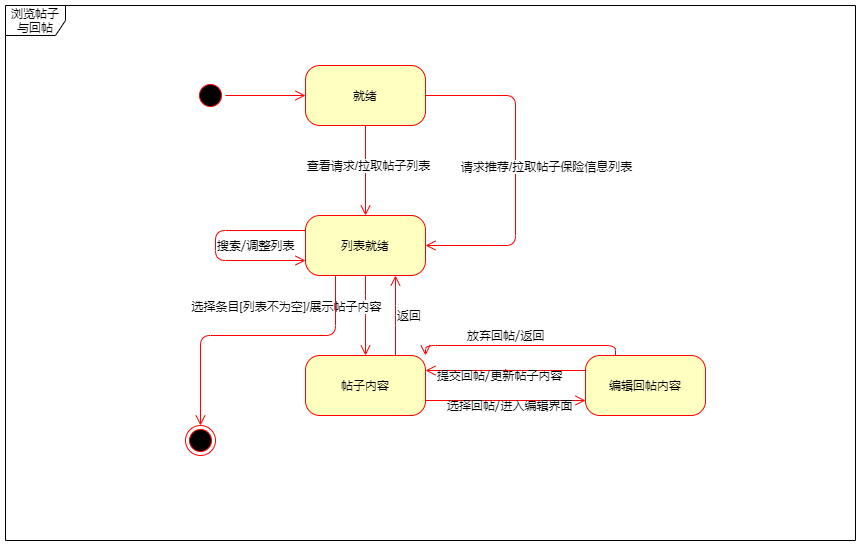
\includegraphics[scale=0.5]{image/2_9状态图.png}
\caption{浏览帖子与回帖状态图}
\label{fig:浏览帖子与回帖状态图}
\end{figure}
图由就绪、列表就绪、帖子内容和编辑回帖内容4种状态组成,需要注意的是编辑回帖内容的状态需要经过查看帖子内容状态。

图\ref{fig:发帖状态图}描述发帖需求中所经过的状态和转移。
\begin{figure}[H]
\centering
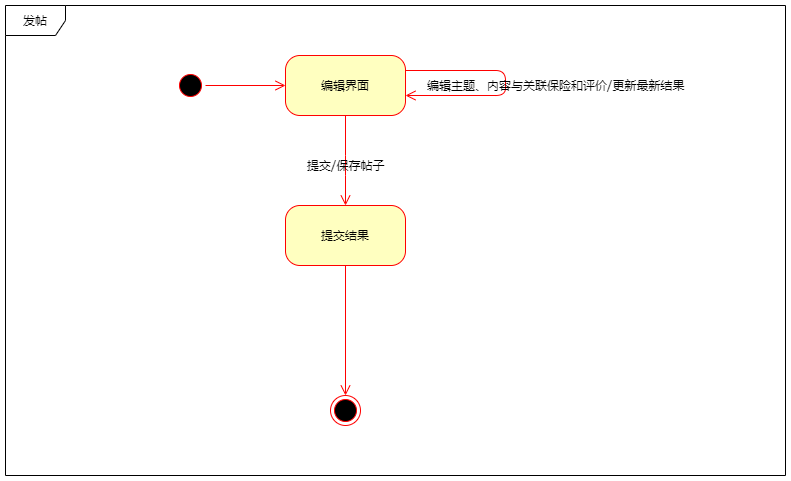
\includegraphics[scale=0.5]{image/2_10状态图.png}
\caption{发帖状态图}
\label{fig:发帖状态图}
\end{figure}
发帖状态图较为简单,在编辑结束后,由编辑界面状态转为提交结果状态,进而结束发帖流程。

\subsection{评价/咨询}

图\ref{fig:用户评价咨询的类图} 描述用户评价咨询的需求相关的实体的属性和交互。
\begin{figure}[H]
\centering
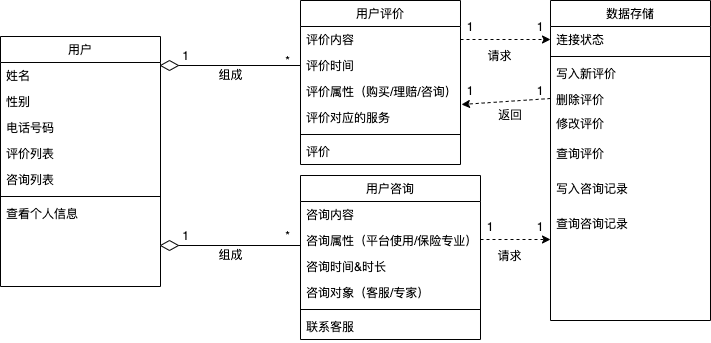
\includegraphics[scale=0.5]{image/3_2类图.png}
\caption{用户评价咨询的类图}
\label{fig:用户评价咨询的类图}
\end{figure}
该类图包含了用户,用户评价,用户咨询,数据存储四个类。用户类中存有用户自身的信息,以及评价列表和咨询列表。评价的类中包含了评价内容,时间,对应的服务等属性。咨询的类中包含了咨询内容,咨询时间和时长,咨询对象等属性。用户的评价和用户咨询的信息都存储在数据库中。\\

图\ref{fig:用户评价和咨询顺序图} 描述用户评价和咨询需求中的实体交互顺序
\begin{figure}[H]
\centering
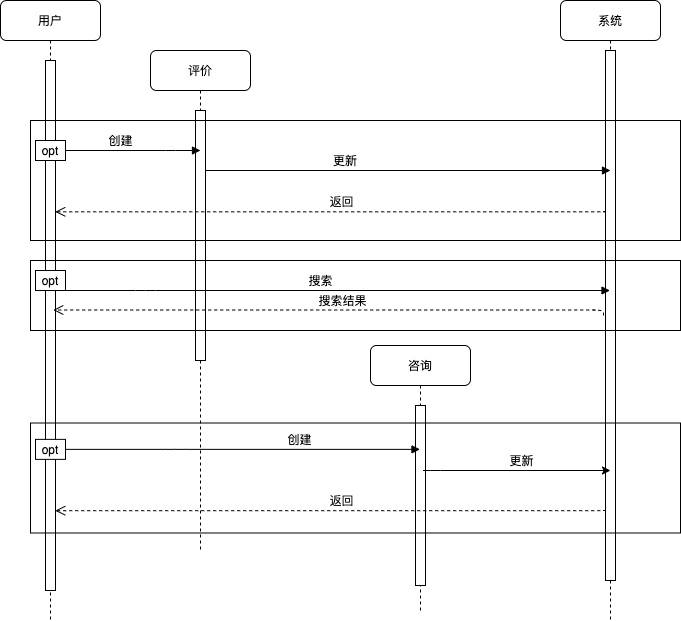
\includegraphics[scale=0.45]{image/3_3顺序图.png}
\caption{用户评价和咨询顺序图}
\label{fig:用户评价和咨询顺序图}
\end{figure}
在用户评价的过程中,用户先创建一个评价类的对象,并且将其加入用户类的评价列表中。用户编写完评价并且提交之后,将评价更新到数据库持久化存储。系统返回用户提交成功的信息。
在用户咨询的过程中,用户先创建一个咨询类的对象,并且将其加入用户类的咨询列表中。用户结束咨询之后,将咨询信息更新到数据库持久化存储。系统返回用户提交成功的信息。
用户可以对自己的评价列表和咨询列表进行关键词搜索或者筛选查询。\\


图\ref{fig:用户评价状态图} 描述用户评价过程中所经过的状态和转移。

\begin{figure}[H]
\centering
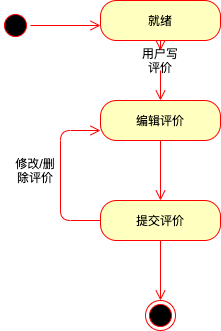
\includegraphics[scale=0.5]{image/3_4状态图.png}
\caption{用户评价状态图}
\label{fig:用户评价状态图}
\end{figure}
用户的主要状态有就绪,编辑评价,提交评价。状态的顺序和顺序图一致。在提交评价之后看到返回提交成功的信息之后结束。\\

图\ref{fig:用户咨询客服状态图} 描述用户咨询客服过程中所经过的状态和转移。

\begin{figure}[H]
\centering
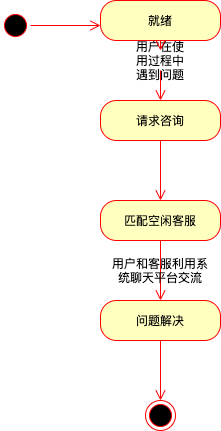
\includegraphics[scale=0.5]{image/3_5状态图.png}
\caption{用户咨询客服状态图}
\label{fig:用户咨询客服状态图}
\end{figure}
用户的主要状态有就绪,请求咨询,匹配空闲客服,问题解决。状态的顺序和顺序图一致。在咨询客服的过程中,用户不需要选择具体某位客服,而是随机进行空闲匹配。问题解决之后,将咨询的记录存在数据库中,最终结束。\\

图\ref{fig:用户咨询领域专家状态图} 描述用户咨询领域专家过程中所经过的状态和转移。

\begin{figure}[H]
\centering
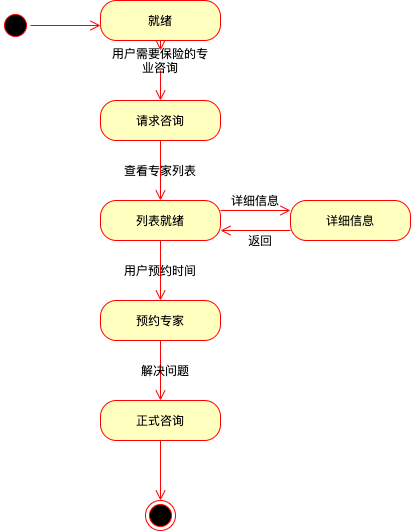
\includegraphics[scale=0.5]{image/3_6状态图.png}
\caption{用户咨询领域专家状态图}
\label{fig:用户咨询领域专家状态图}
\end{figure}
用户的主要状态有就绪,请求咨询,专家列表就绪,预约专家,正式咨询这几个状态。用户需要先查看专家列表选择合适的专家,用户在查看列表的时候,可以选择查看专家的详细信息。选择合适的专家之后再进行预约咨询,咨询结束后将咨询记录存在数据库中,最终结束。\\

\subsection{产品信息管理}

图\ref{fig:产品信息管理类图} 描述产品信息管理相关的实体的属性和交互。
\begin{figure}[H]
\centering
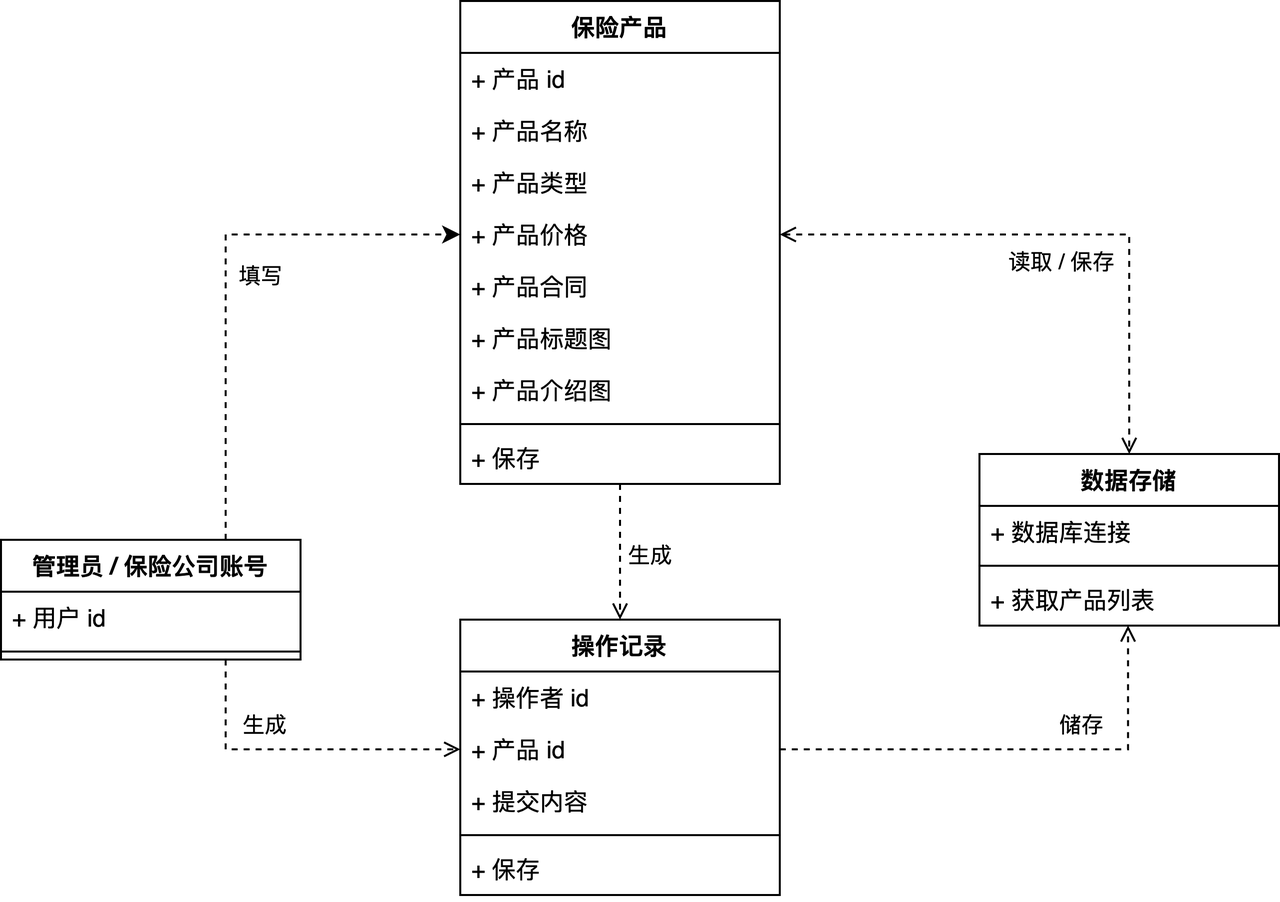
\includegraphics[scale=0.25]{image/4_3类图.png}
\caption{产品信息管理的类图}
\label{fig:产品信息管理类图}
\end{figure}
该类图包含了用户、保险产品、操作记录、数据存储四个类和实体。用户类中储存了用户身份的相关信息,保险产品类储存了产品详情,用户的新增、修改操作会被记录在操作日志类中,数据存储类负责持久化存储数据。\\

图\ref{fig:产品信息管理顺序图} 描述产品信息管理实体交互顺序。
\begin{figure}[H]
\centering
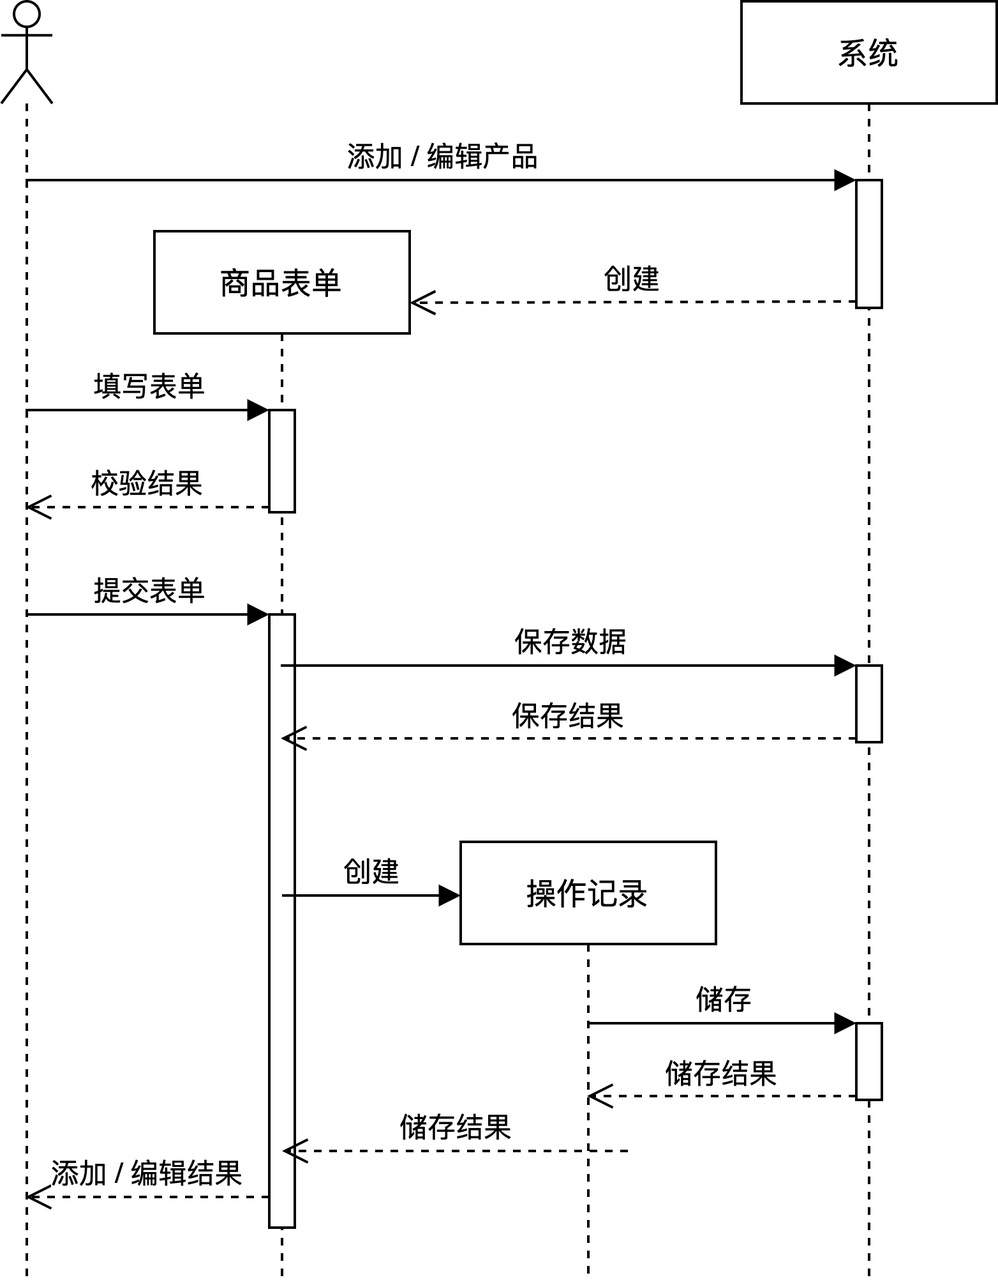
\includegraphics[scale=0.2]{image/4_4顺序图.png}
\caption{产品信息管理顺序图}
\label{fig:产品信息管理顺序图}
\end{figure}
用户发起新建、修改请求,系统返回表单供用户填写,并即使给出校验结果,在用户提交表单后,系统进行持久化存储,同时记录操作日志。\\

图\ref{fig:产品信息管理状态图} 描述产品信息管理状态和转移。
\begin{figure}[H]
\centering
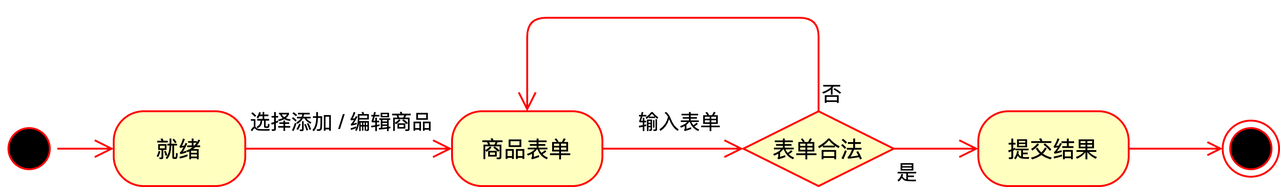
\includegraphics[scale=0.3]{image/4_5状态图.png}
\caption{产品信息管理状态图}
\label{fig:产品信息管理状态图}
\end{figure}
主要状态有就绪,表单填写,提交结果。用户请求表单之后,可以填写商品信息,校验通过后,提交到数据库中持久化存储,并展示提交结果。状态的顺序和顺序图一致。\\

\subsection{查看产品购买记录}

图\ref{fig:查看产品购买记录类图} 描述查看产品购买记录相关的实体的属性和交互。
\begin{figure}[H]
\centering
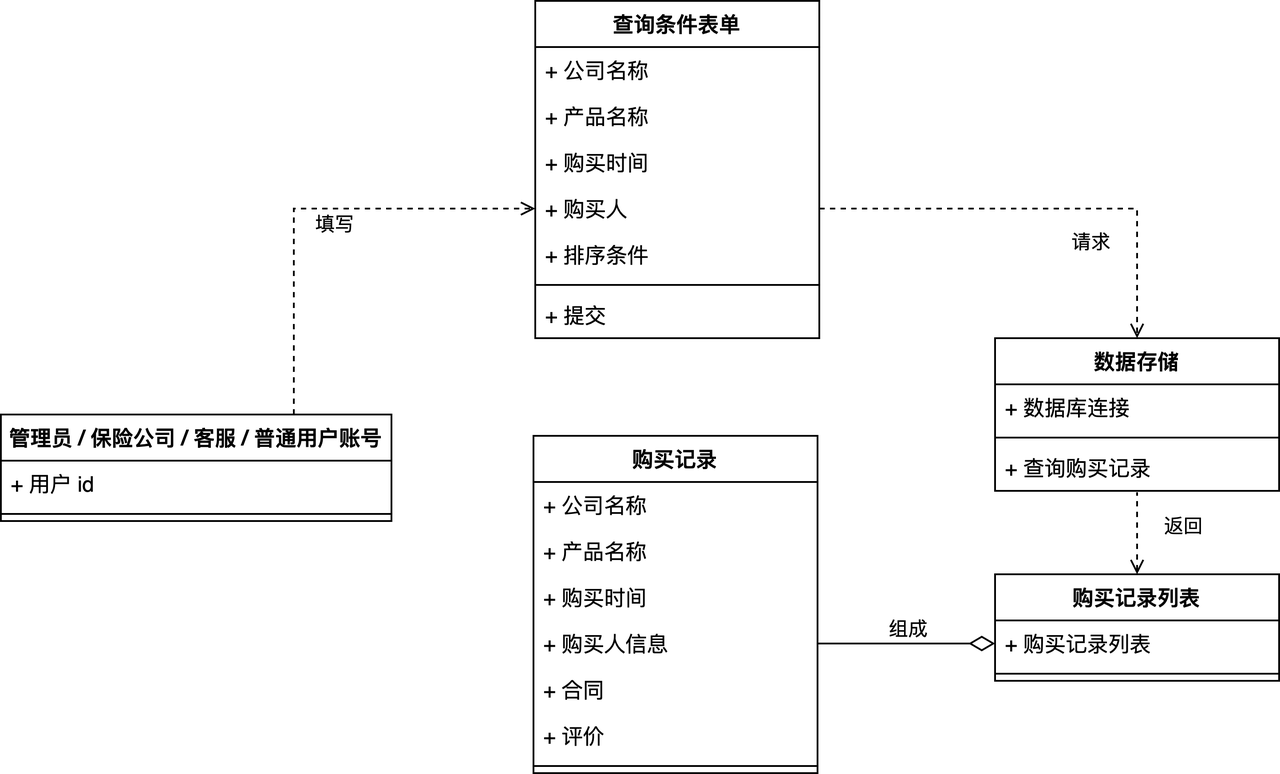
\includegraphics[scale=0.3]{image/4_6类图.png}
\caption{查看产品购买记录的类图}
\label{fig:查看产品购买记录类图}
\end{figure}
该类图包含了用户、查询条件表单、购买记录列表、购买记录、数据存储五个类和实体。用户类中储存了用户身份的相关信息,查询条件表单包含了要搜索的购买记录的信息、排序方式,由数据储存解析查询条件表单并返回购买记录列表,其中以一定顺序包含了符合条件的购买记录。\\

图\ref{fig:查看产品购买记录顺序图} 描述查看产品购买记录实体交互顺序。
\begin{figure}[H]
\centering
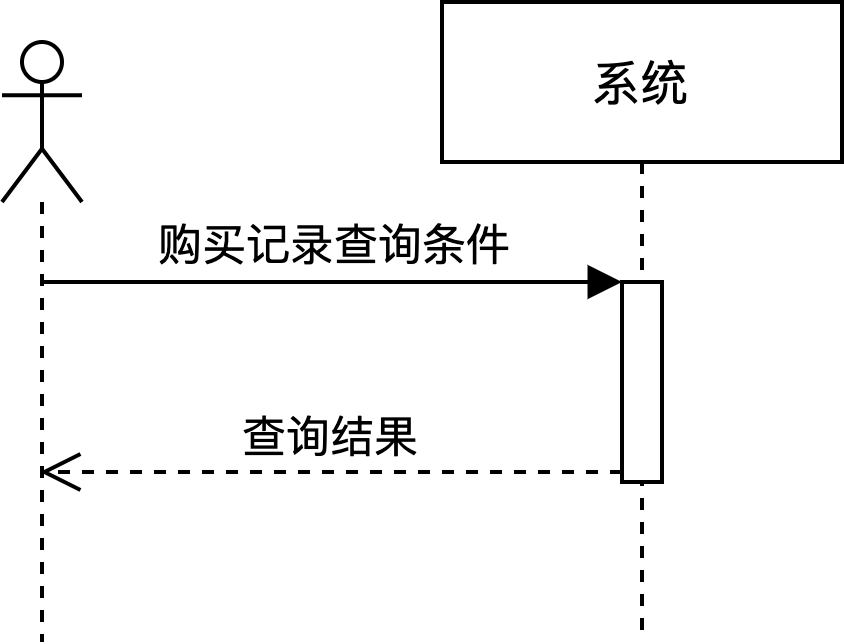
\includegraphics[scale=0.2]{image/4_7顺序图.png}
\caption{查看产品购买记录顺序图}
\label{fig:查看产品购买记录顺序图}
\end{figure}
用户提交查询条件表单,系统返回查询结果。\\

图\ref{fig:查看产品购买记录状态图} 描述查看产品购买记录状态和转移。
\begin{figure}[H]
\centering
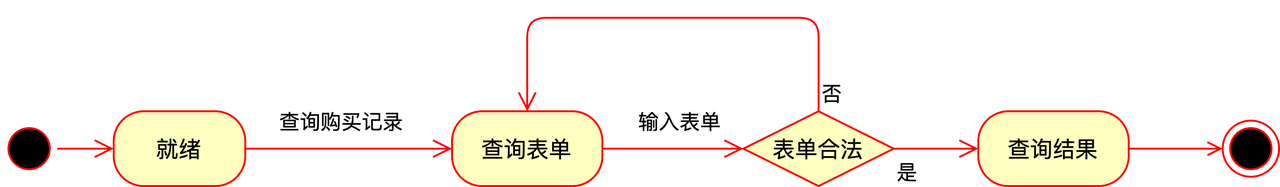
\includegraphics[scale=0.3]{image/4_8状态图.png}
\caption{查看产品购买记录状态图}
\label{fig:查看产品购买记录状态图}
\end{figure}
主要状态有就绪,表单填写,查询结果。用户可以在表单中填写过滤条件、排序条件,校验通过后,系统在数据库中查找信息,并展示查询结果。状态的顺序和顺序图一致。\\


\subsection{账号管理}
图\ref{fig:账号管理的类图} 描述账号管理相关的实体的属性和交互。
\begin{figure}[H]
\centering
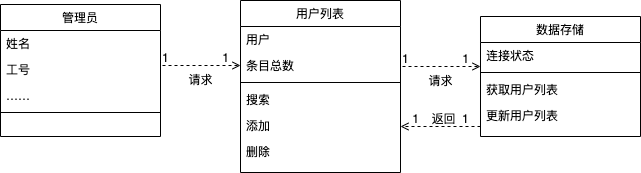
\includegraphics[scale=0.5]{image/5_1类图.png}
\caption{账号管理的类图}
\label{fig:账号管理的类图}
\end{figure}
该类图包含了管理员,用户列表和数据存储三个类和实体。管理员的类中存储了管理员自身的信息,如姓名、工号等。用户列表存所有的用户信息,和条目总数,管理员可以对用户列表进行增删改查的操作。修改完成之后再更新到数据库中。\\

图\ref{fig:账号管理顺序图} 描述用账号管理实体交互顺序。
\begin{figure}[H]
\centering
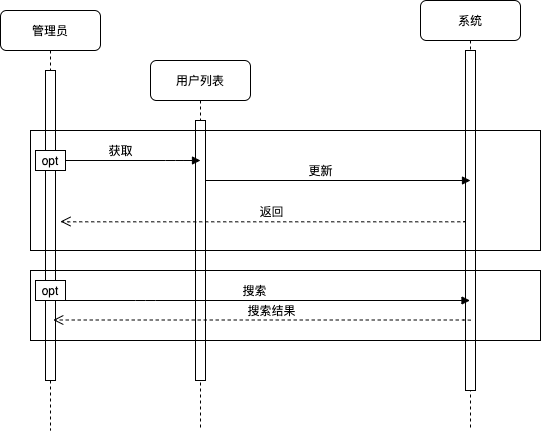
\includegraphics[scale=0.5]{image/5_2顺序图.png}
\caption{账号管理顺序图}
\label{fig:账号管理顺序图}
\end{figure}
管理员可以从数据库里直接筛选查询用户。如果要更新数据库中的用户信息,需要先获取用户列表这一实体,在用户列表内修改之后再持久化到系统中。\\

图\ref{fig:账号管理状态图} 描述账号管理状态和转移。
\begin{figure}[H]
\centering
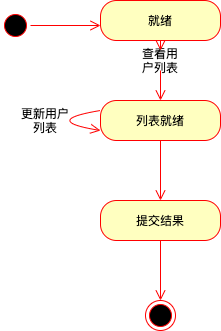
\includegraphics[scale=0.5]{image/5_3状态图.png}
\caption{账号管理状态图}
\label{fig:账号管理状态图}
\end{figure}
主要状态有就绪,列表就绪,提交结果。列表就绪之后,管理员可以对列表进行增删改查的操作,然后提交到数据库中持久化存储。状态的顺序和顺序图一致。\\

\section{跟踪矩阵}

\subsection{需求列表}
\begin{enumerate}[label=BR\arabic*.]
  \item 在第一版应用之后的3个月内,将用户的平均保险挑选时间降低50\%
  \item 在在第一版应用之后的3个月内,将用户的平均保险业务办理时间降低30\%
  \item 在第一版应用之后的6个月内,将合作保险公司的保险销售额提升15\%
  \item 在第一版应用之后的6个月内,用户对在本系统中所办理的保险业务的好评率达到85\%
  \item 在第一版应用之后的6个月内,与本平台进行合作的保险公司数量达到当前市场中的80\%(以市场份额作为基准)
\end{enumerate}

\begin{enumerate}[label=UR1.]
  \item 申请理赔
\end{enumerate}
\begin{enumerate}[label=SR1.]
  \item 
  \begin{enumerate}[label=\arabic*).]
    \item 系统提供入口供用户上传资料
    \item 系统提供入口供管理员审核
    \item 系统允许管理员和保险公司之间传递材料
    \item 当用户提起申诉时,系统能够记录此次申诉过程和结果
  \end{enumerate}
\end{enumerate}

\begin{enumerate}[label=UR2.]
  \item 购买保险
\end{enumerate}
\begin{enumerate}[label=SR2.]
  \item 
  \begin{enumerate}[label=\arabic*).]
    \item 系统能够展示各个种类的保险
    \item 系统允许用户选择保险购买
    \item 当用户选择购买时,系统应请求第三方接口负责支付
    \item 系统能够接收第三方接口返回的支付结果信息
    \item 系统能够将购买结果展示给用户
    \item 系统能够记录此次购买的结果
  \end{enumerate}
\end{enumerate}

\begin{enumerate}[label=UR3.]
  \item 联系客服
\end{enumerate}
\begin{enumerate}[label=SR3.]
  \item 
  \begin{enumerate}[label=\arabic*).]
    \item 系统能展示历史问题列表
    \item 系统允许用户描述自己的问题
    \item 系统允许用户和人工客服进行交互
    \item 系统能够记录此次交流过程和结果
  \end{enumerate}
\end{enumerate}

\begin{enumerate}[label=UR4.]
  \item 浏览保险信息
\end{enumerate}
\begin{enumerate}[label=SR4.]
  \item 
  \begin{enumerate}[label=\arabic*).]
    \item 系统可以让用户查看保险信息
    \item 用户查看保险信息列表时,系统可以将保险信息按评价从高到低分页给用户查看
    \item 用户选择列表中的某条保险信息条目时,系统可以将保险的名称、所属企业、类别、详细条款、价格、相关评价等信息呈现给用户
  \end{enumerate}
\end{enumerate}
\begin{enumerate}[label=SR5.]
  \item 
  \begin{enumerate}[label=\arabic*).]
    \item 系统可以给用户推荐适合的保险信息列表
    \item 用户查看推荐的保险信息列表时,系统可以将保险信息按推荐系数从高到低分页给用户查看
  \end{enumerate}
\end{enumerate}
\begin{enumerate}[label=SR6.]
  \item 
  \begin{enumerate}[label=\arabic*).]
    \item 系统可以让用户筛选保险信息列表
    \item 用户输入关键字或者选择保险类别,系统通过筛选条件过滤不包含关键字或非选中类别的保险信息,更新保险信息列表
  \end{enumerate}
\end{enumerate}
\begin{enumerate}[label=SR7.]
  \item 
  \begin{enumerate}[label=\arabic*).]
    \item 系统可以让用户对保险信息进行对比
    \item 系统呈现保险信息列表后,用户选择两项要对比的保险信息条目,系统对齐两条保险信息的各个属性,呈现给用户
  \end{enumerate}
\end{enumerate}

\begin{enumerate}[label=UR5.]
  \item 浏览论坛
\end{enumerate}
\begin{enumerate}[label=SR8.]
  \item 
  \begin{enumerate}[label=\arabic*).]
    \item 系统可以让用户查看论坛帖子
    \item 用户查看论坛帖子列表时,系统可以将帖子按更新时间从近到远分页给用户查看
    \item 用户选择列表中的某项帖子条目时,系统可以将保险的名称、所属企业、类别、详细条款、价格、相关评价等信息呈现给用户
  \end{enumerate}
\end{enumerate}
\begin{enumerate}[label=SR9.]
  \item 
  \begin{enumerate}[label=\arabic*).]
    \item 系统可以给用户推荐适合的帖子列表
    \item 用户查看推荐的帖子列表时,系统可以将帖子按推荐系数从高到低分页给用户查看
  \end{enumerate}
\end{enumerate}
\begin{enumerate}[label=SR10.]
  \item 
  \begin{enumerate}[label=\arabic*).]
    \item 系统可以让用户筛选帖子列表
    \item 用户输入关键字,系统通过筛选条件过滤不包含关键字的帖子,更新帖子列表
  \end{enumerate}
\end{enumerate}

\begin{enumerate}[label=UR6.]
  \item 发帖
\end{enumerate}
\begin{enumerate}[label=SR11.]
  \item 
  \begin{enumerate}[label=\arabic*).]
    \item 系统可以让用户发帖
    \item 用户通过系统发帖后,系统能正确将信息保存到数据库
  \end{enumerate}
\end{enumerate}

\begin{enumerate}[label=UR7.]
  \item 回帖
\end{enumerate}
\begin{enumerate}[label=SR12.]
  \item 
  \begin{enumerate}[label=\arabic*).]
    \item 系统可以让用户回帖
    \item 用户通过系统回帖后,系统能正确将信息保存到数据库,更新该帖子的数据
  \end{enumerate}
\end{enumerate}

\begin{enumerate}[label=UR8.]
  \item 查看评价
\end{enumerate}
\begin{enumerate}[label=SR13.]
  \item 
  \begin{enumerate}[label=\arabic*).]
    \item 系统可以让普通用户看到当前服务下(购买/理赔/咨询)所有用户的评价,可按照热度或者时间顺序分页显示
    \item 系统允许普通用户搜索某一条评价
    \item 系统允许普通用户对评价进行筛选(根据时间,有无图片,关键词等)
  \end{enumerate}
\end{enumerate}

\begin{enumerate}[label=UR9.]
  \item 用户进行评价
\end{enumerate}
\begin{enumerate}[label=SR14.]
  \item 
  \begin{enumerate}[label=\arabic*).]
    \item 系统可以让用户在评价的文字中插入视频和图片
    \item 系统需要让用户在提交评价之前打上等级
    \item 系统可以开放对用户评价的评论功能,允许保险公司,和其他用户在下方评论
    \item 系统可以让用户修改之前的评价
    \item 系统可以让用户删除之前的评价
    \item 系统将用户的评价持久化到数据库
  \end{enumerate}
\end{enumerate}

\begin{enumerate}[label=UR10.]
  \item 平台使用咨询
\end{enumerate}
\begin{enumerate}[label=SR15.]
  \item 
  \begin{enumerate}[label=\arabic*).]
    \item 用户向客服发送咨询之后,系统自动匹配空闲的客服为用户解答
    \item 系统支持客服以语音,视频,图片文字的方式和用户交流
    \item 系统将用户的咨询记录持久化到数据库,方便用户之后查看
  \end{enumerate}
\end{enumerate}

\begin{enumerate}[label=UR11.]
  \item 保险专业咨询
\end{enumerate}
\begin{enumerate}[label=SR16.]
  \item 
  \begin{enumerate}[label=\arabic*).]
    \item 系统自动为用户推荐适合用户的专家列表(擅长某一方面的保险产品的专家)
    \item 系统可以让用户通过专家列表了解每一个专家的特点,方便选择
    \item 系统为用户显示当前专家的空闲时间供用户预约
    \item 当用户开始咨询的时候,系统开始计时,方便之后结算费用
    \item 系统将用户的咨询记录持久化到数据库,方便用户之后查看
  \end{enumerate}
\end{enumerate}

\begin{enumerate}[label=UR12.]
  \item 产品信息管理
\end{enumerate}
\begin{enumerate}[label=SR17.]
  \item 
  \begin{enumerate}[label=\arabic*).]
    \item 系统允许管理员、保险公司新建、修改产品
    \item 用户在提交时需要输入:标题大图、介绍长图、保险名称、保险类型、保险价格、保险合同样本等信息
    \item 系统应将操作进行记录并持久化储存,方便以后查询
  \end{enumerate}
\end{enumerate}

\begin{enumerate}[label=UR13.]
  \item 查看产品购买记录
\end{enumerate}
\begin{enumerate}[label=SR18.]
  \item 
  \begin{enumerate}[label=\arabic*).]
    \item 系统允许管理员、保险公司、客服查看产品购买记录
    \item 系统应展示保险名称、购买时间、购买人基本信息、所签合同、评价等信息
    \item 用户可以根据保险公司、保险名称、购买时间、购买人等条件进行筛选
    \item 用户可以按照购买时间、投保时长、投保金额、评分等信息进行排序
    \item 保险公司只可查询本公司产品的购买记录
    \item 普通用户只能看到产品的购买时间、评价信息
  \end{enumerate}
\end{enumerate}

\begin{enumerate}[label=UR14.]
  \item 账号管理
\end{enumerate}
\begin{enumerate}[label=SR19.]
  \item 
  \begin{enumerate}[label=\arabic*).]
    \item 系统可以让管理员查看所有用户的账号
    \item 管理员可以创建或删除某一个用户的账号
    \item 系统将用户的信息都持久化到数据库中保存
  \end{enumerate}
\end{enumerate}

\subsection{跟踪矩阵}

{
\tiny
\centering
  \begin{longtable}{|P{4em}|P{4em}|P{2em}|P{2em}|P{2em}|P{1em}|P{3em}|P{3em}|P{4em}|P{4em}|P{2em}|P{2em}|P{3em}|P{3em}|P{4em}|P{4em}|}
    \hline
    \multicolumn{3}{|c}{\multirow{2}*{原始信息}} & \multicolumn{7}{|c}{过程信息}       & \multicolumn{3}{|c}{\multirow{2}*{处理信息}} & \multicolumn{3}{|c|}{\multirow{2}*{变更信息}}                                                                                                                                                                                    \\
    \cline{4-10}
    \multicolumn{3}{|c}{~}                       & \multicolumn{3}{|c}{需求是否可实现} & \multicolumn{4}{|c}{需求是否符合规划目标}    & \multicolumn{3}{|c}{~}                        & \multicolumn{3}{|c|}{~}                                                                                                                                                          \\
    \hline
    需求编号                                     & 需求类别                            & 需求来源                                     & 具有难度                                      & 可行性                  & 风险 & 改善产品功能 & 改善产品性能 & 增加用户满意度 & 增加产品竞争力 & 是否实现 & 优先级 & 未实现原因 & 是否出现变更 & 变更基线       & 变更记录       \\
    \hline
    \endfirsthead
      \multicolumn{16}{r}{续表}\\
  \multicolumn{16}{c}{(接上页)}\\
    \hline
    \multicolumn{3}{|c}{\multirow{2}*{原始信息}} & \multicolumn{7}{|c}{过程信息}       & \multicolumn{3}{|c}{\multirow{2}*{处理信息}} & \multicolumn{3}{|c|}{\multirow{2}*{变更信息}}                                                                                                                                                                                    \\
    \cline{4-10}
    \multicolumn{3}{|c}{~}                       & \multicolumn{3}{|c}{需求是否可实现} & \multicolumn{4}{|c}{需求是否符合规划目标}    & \multicolumn{3}{|c}{~}                        & \multicolumn{3}{|c|}{~}                                                                                                                                                          \\
    \hline
    需求编号                                     & 需求类别                            & 需求来源                                     & 具有难度                                      & 可行性                  & 风险 & 改善产品功能 & 改善产品性能 & 增加用户满意度 & 增加产品竞争力 & 是否实现 & 优先级 & 未实现原因 & 是否出现变更 & 变更基线       & 变更记录       \\
    \hline
  \endhead
    \hline
  \multicolumn{16}{c}{(接下页)}
  \endfoot
\hline
  \endlastfoot
  BR1                                          & 业务需求                            & 客户                                         & 否                                            & 可行                    & 无   & 是           & 是           & 是             & 是             & 实现     & 4      &            & 否           &                 &                        \\
  \hline
  BR2                                          & 业务需求                            & 客户                                         & 否                                            & 可行                    & 无   & 是           & 是           & 是             & 是             & 实现     & 4      &            & 是           & 见需求文档 BR2  & 50\% 修改为 30\%       \\
  \hline
  BR3                                          & 业务需求                            & 市场                                         & 否                                            & 可行                    & 无   & 否           & 否           & 是             & 是             & 实现     & 4      &            & 否           &                 &                        \\
  \hline
  BR4                                          & 业务需求                            & 市场                                         & 否                                            & 可行                    & 无   & 否           & 否           & 是             & 是             & 实现     & 3      &            & 否           &                 &                        \\
  \hline
  BR5                                          & 业务需求                            & 市场                                         & 是                                            & 可行                    & 无   & 是           & 否           & 是             & 是             & 实现     & 2      &            & 否           &                 &                        \\
  \hline
  UR1                                          & 用户需求                            & 客户                                         & 是                                            & 可行                    & 有   & 是           & 否           & 是             & 是             & 实现     & 2      &            & 否           &                 &                        \\
  \hline
  SR1                                          & 系统需求                            & 客户                                         & 是                                            & 可行                    & 有   & 是           & 否           & 是             & 是             & 实现     & 2      &            & 否           &                 &                        \\
  \hline
  UR2                                          & 用户需求                            & 客户                                         & 否                                            & 可行                    & 无   & 是           & 否           & 是             & 否             & 实现     & 1      &            & 否           &                 &                        \\
  \hline
  SR2                                          & 系统需求                            & 客户                                         & 否                                            & 可行                    & 无   & 是           & 否           & 是             & 否             & 实现     & 1      &            & 否           &                 &                        \\
  \hline
  UR3                                          & 用户需求                            & 客户                                         & 否                                            & 可行                    & 无   & 是           & 否           & 是             & 是             & 实现     & 1      &            & 否           &                 &                        \\
  \hline
  SR3                                          & 系统需求                            & 客户                                         & 否                                            & 可行                    & 无   & 是           & 否           & 是             & 是             & 实现     & 1      &            & 否           &                 &                        \\
  \hline
  UR4                                          & 用户需求                            & 客户                                         & 否                                            & 可行                    & 无   & 是           & 否           & 是             & 否             & 实现     & 1      &            & 否           &                 &                        \\
  \hline
  SR4                                          & 系统需求                            & 客户                                         & 否                                            & 可行                    & 无   & 是           & 否           & 是             & 否             & 实现     & 1      &            & 否           &                 &                        \\
  \hline
  SR5                                          & 系统需求                            & 客户                                         & 是                                            & 可行                    & 无   & 是           & 否           & 是             & 是             & 实现     & 2      &            & 否           &                 &                        \\
  \hline
  SR6                                          & 系统需求                            & 客户                                         & 否                                            & 可行                    & 无   & 是           & 否           & 是             & 否             & 实现     & 1      &            & 否           &                 &                        \\
  \hline
  SR7                                          & 系统需求                            & 客户                                         & 否                                            & 可行                    & 无   & 是           & 否           & 是             & 是             & 实现     & 2      &            & 是           & 无              & 新增需求               \\
  \hline
  UR5                                          & 用户需求                            & 客户                                         & 否                                            & 可行                    & 无   & 是           & 否           & 是             & 是             & 实现     & 2      &            & 否           &                 &                        \\
  \hline
  SR8                                          & 系统需求                            & 客户                                         & 否                                            & 可行                    & 无   & 是           & 否           & 是             & 是             & 实现     & 2      &            & 否           &                 &                        \\
  \hline
  SR9                                          & 系统需求                            & 客户                                         & 是                                            & 可行                    & 无   & 是           & 否           & 是             & 是             & 实现     & 3      &            & 是           & 无              & 新增需求               \\
  \hline
  SR10                                         & 系统需求                            & 客户                                         & 否                                            & 可行                    & 无   & 是           & 否           & 是             & 是             & 实现     & 2      &            & 否           &                 &                        \\
  \hline
  UR6                                          & 用户需求                            & 客户                                         & 否                                            & 可行                    & 有   & 是           & 否           & 是             & 是             & 实现     & 2      &            & 否           &                 &                        \\
  \hline
  SR11                                         & 系统需求                            & 客户                                         & 否                                            & 可行                    & 有   & 是           & 否           & 是             & 是             & 实现     & 2      &            & 否           &                 &                        \\
  \hline
  UR7                                          & 用户需求                            & 客户                                         & 否                                            & 可行                    & 有   & 是           & 否           & 是             & 是             & 实现     & 2      &            & 否           &                 &                        \\
  \hline
  SR12                                         & 系统需求                            & 客户                                         & 否                                            & 可行                    & 有   & 是           & 否           & 是             & 是             & 实现     & 2      &            & 否           &                 &                        \\
  \hline
  UR8                                          & 用户需求                            & 客户                                         & 否                                            & 可行                    & 无   & 是           & 否           & 是             & 是             & 实现     & 1      &            & 是           & 见需求文档 UR8  & 新增评价搜索           \\
  \hline
  SR13                                         & 系统需求                            & 客户                                         & 否                                            & 可行                    & 无   & 是           & 否           & 是             & 是             & 实现     & 1      &            & 否           &                 &                        \\
  \hline
  UR9                                          & 用户需求                            & 客户                                         & 否                                            & 可行                    & 无   & 是           & 否           & 是             & 是             & 实现     & 1      &            & 否           &                 &                        \\
  \hline
  SR14                                         & 系统需求                            & 客户                                         & 否                                            & 可行                    & 无   & 是           & 否           & 是             & 是             & 实现     & 1      &            & 是           & 见需求文档 SR14 & 允许用户编辑、修改评价 \\
  \hline
  UR10                                         & 用户需求                            & 客户                                         & 否                                            & 可行                    & 无   & 是           & 否           & 是             & 是             & 实现     & 1      &            & 否           &                 &                        \\
  \hline
  SR15                                         & 系统需求                            & 客户                                         & 否                                            & 可行                    & 无   & 是           & 否           & 是             & 是             & 实现     & 1      &            & 否           &                 &                        \\
  \hline
  UR11                                         & 用户需求                            & 市场                                         & 否                                            & 可行                    & 无   & 是           & 否           & 是             & 是             & 实现     & 2      &            & 否           &                 &                        \\
  \hline
  SR16                                         & 系统需求                            & 市场                                         & 否                                            & 可行                    & 无   & 是           & 否           & 是             & 是             & 实现     & 2      &            & 否           &                 &                        \\
  \hline
  UR12                                         & 用户需求                            & 客户                                         & 否                                            & 可行                    & 无   & 是           & 是           & 否             & 否             & 实现     & 1      &            & 否           &                 &                        \\
  \hline
  SR17                                         & 系统需求                            & 客户                                         & 否                                            & 可行                    & 无   & 是           & 是           & 否             & 否             & 实现     & 1      &            & 否           &                 &                        \\
  \hline
  UR13                                         & 用户需求                            & 客户                                         & 否                                            & 可行                    & 有   & 是           & 是           & 是             & 是             & 实现     & 1      &            & 否           &                 &                        \\
  \hline
  SR18                                         & 系统需求                            & 客户                                         & 否                                            & 可行                    & 有   & 是           & 是           & 是             & 是             & 实现     & 1      &            & 否           &                 &                        \\
  \hline
  UR14                                         & 用户需求                            & 客户                                         & 否                                            & 可行                    & 无   & 是           & 是           & 否             & 否             & 实现     & 1      &            & 否           &                 &                        \\
  \hline
  SR19                                         & 系统需求                            & 客户                                         & 否                                            & 可行                    & 无   & 是           & 是           & 否             & 否             & 实现     & 1      &            & 否           &                 &                        \\
  \end{longtable}
  }

\end{document}